\documentclass[sigconf]{acmart} %anonymous, 
\usepackage{graphicx} % Required for inserting images
\usepackage{subcaption}
\usepackage{siunitx}
\usepackage{listings}
\usepackage{xspace}
\usepackage[]{hyperref}
\usepackage{circledsteps}
\usepackage{float}
\usepackage{enumitem}
\usepackage{mathtools}
\usepackage{algorithm} 
\usepackage{algpseudocode} 
\usepackage[export]{adjustbox}% http://ctan.org/pkg/adjustbox
\usepackage{graphicx}
\usepackage{titlesec}

\usepackage{mdframed}
\mdfsetup{nobreak=true}
\usepackage{fancyhdr}

\renewcommand{\sectionautorefname}{Section}
\def\algorithmautorefname{Algorithm}
\renewcommand{\subsectionautorefname}{Section}
\renewcommand{\subsubsectionautorefname}{Section}
\renewcommand{\figureautorefname}{Figure}

\titleformat*{\subsubsection}{\bfseries}

\captionsetup{compatibility=false}




\usepackage[many,theorems,skins,breakable]{tcolorbox}
\definecolor{tcbcolback}{RGB}{245,243,253}
\definecolor{tcbcolbox}{RGB}{254 218 173}
\definecolor{tcbcolframe}{RGB}{245,243,253}
\newtcolorbox{visionbox}[2][]{%
    colback=white!12,
    % colback=tcbcolbox!100,
    coltitle=black,
    colframe=teal!50,
    fonttitle=\bfseries,
    title=#2, 
    sharp corners,
    rounded corners=southeast,
    boxrule=0pt,
    enhanced,
    drop fuzzy shadow,
    #1, 
    top=3pt,bottom=2pt,left=3pt,right=3pt
    }


%% \BibTeX command to typeset BibTeX logo in the docs
\AtBeginDocument{%
  \providecommand\BibTeX{{%
    Bib\TeX}}}

% \newcounter{todonumber}
% \stepcounter{todonumber}
% \newcommand{\todo}[1]{\textcolor{red}{Todo\#\arabic{todonumber}\stepcounter{todonumber}: #1}}
% % \newcommand\abel[1]{\textcolor{green}{(A: #1)}}
% % \newcommand\prash[1]{\textcolor{blue}{(P: #1)}}
% \newcommand\lilly[1]{\textcolor{orange}{(L: #1)}}
% % \newcommand\walid[1]{\textcolor{red}{(W: #1)}}

%% complete the rights form.
\setcopyright{acmlicensed}
\copyrightyear{2025}
\acmYear{2025}
\acmDOI{XXXXXXX.XXXXXXX}

%% These commands are for a PROCEEDINGS abstract or paper.
%%
%%  Uncomment \acmBooktitle if the title of the proceedings is different
%%  from ``Proceedings of ...''!
%%
%%\acmBooktitle{Woodstock '18: ACM Symposium on Neural Gaze Detection,
%%  June 03--05, 2018, Woodstock, NY}
% \acmISBN{978-1-4503-XXXX-X/18/06}

% \settopmatter{printacmref=false}
% \renewcommand\footnotetextcopyrightpermission[1] 

% \title{CarbonEdge: A Carbon-Aware Control Plane for Edge-Native Applications}
\title{CarbonEdge: Leveraging Mesoscale Spatial Carbon-Intensity Variations for Low Carbon Edge Computing}
% \title{Leveraging Carbon-Intensity Variations Across Micro Regions for Edge Computing}

\renewcommand{\shorttitle}{CarbonEdge}
%Leveraging Carbon-Intensity Variations Across Micro Regions for Edge Computing
%No Contrast: Overhead-free Carbon-aware Spatial Shifting for Edge Computing
%

% \author{Paper Type: Regular, Paper ID: 51}

\author{Li Wu}
\affiliation{
  \institution{University of Massachusetts Amherst}
  \country{USA}
}
\author{Walid A. Hanafy}
\affiliation{
  \institution{University of Massachusetts Amherst}
  \country{USA}
}
\author{Abel Souza}
\affiliation{
  \institution{University of California, Santa Cruz}
  \country{USA}
}
\author{Khai Nguyen}
\affiliation{
  \institution{University of Massachusetts Amherst}
  \country{USA}
}
\author{Jan Harkes}
\affiliation{
  \institution{Carnegie Mellon University}
  \country{USA}
}
\author{David Irwin}
\affiliation{
  \institution{University of Massachusetts Amherst}
  \country{USA}
}
\author{Mahadev Satyanarayanan}
\affiliation{
  \institution{Carnegie Mellon University}
  \country{USA}
}
\author{Prashant Shenoy}
\affiliation{
  \institution{University of Massachusetts Amherst}
  \country{USA}
}

% \author{Li Wu, Walid A. Hanafy, Abel Souza, Khai Nguyen, Jan Harkes, David Irwin, \\ Mahadev Satyanarayanan, Prashant Shenoy}

% \affiliation{
%   \institution{University of Massachusetts Amherst, USA}
%   \institution{University of California, Santa Cruz, USA}
%   \institution{Carnegie Mellon University, USA}
% }

% \author{Li Wu\textsuperscript{1}, Walid A. Hanafy\textsuperscript{1}, Abel Souza\textsuperscript{2}, Khai Nguyen\textsuperscript{1}, Jan Harkes\textsuperscript{3}, David Irwin\textsuperscript{1}, \\ Mahadev Satyanarayanan\textsuperscript{3}, Prashant Shenoy\textsuperscript{1}}

% \affiliation{
%   \textsuperscript{1}University of Massachusetts Amherst, USA \\
%   \textsuperscript{2}University of California, Santa Cruz, USA \\
%   \textsuperscript{3}Carnegie Mellon University, USA
% }




% \date{April 2024}

\settopmatter{printacmref=false}
% \setcopyright{none}
% \pagestyle{empty}

\pagestyle{fancy}
\fancyhead[R]{\theauthor} % Show the first author on all pages

\renewcommand\footnotetextcopyrightpermission[1]{} 

% \settopmatter{printacmref=false} % Removes the ACM reference information
% \setcopyright{none} % Removes copyright information
% \pagestyle{empty} % Optional: Removes page numbers if needed


\def\carbonunit{g$\cdot$CO$_2$eq/kWh\xspace}
\def\emissionunit{g$\cdot$CO$_2$eq\xspace}
\def\emissionkgunit{kg$\cdot$CO$_2$eq\xspace}
\def\emissiontunit{t$\cdot$CO$_2$eq\xspace}
\def\proposedsystem{\textit{CarbonEdge}\xspace}
%Come up with a better name
% \def\realsystem{\texttt{CarbonEdge-REAL}\xspace}

%\def \simulationsystem{\texttt{CarbonEdge-SIM}\xspace}

\def\latencyaware{\texttt{Latency-aware}\xspace}
\def\energyaware{\texttt{Energy-aware}\xspace}
\def\intensityaware{\texttt{Intensity-aware}\xspace}


\renewcommand{\sectionautorefname}{Section}

%%%% Start: By walid to squeeze all spaced
\captionsetup{skip=1pt}
\captionsetup[subfigure]{skip=0pt}
\setlength{\textfloatsep}{3pt}

\titlespacing{\section}{0pt}{*0.7}{*0.4} % Adjusts space above and below section
\titlespacing{\subsection}{0pt}{*0.2}{*0.1} % Adjusts space above and below section
\titlespacing{\subsubsection}{0pt}{*0}{*0} % Adjusts space above and below section
\titleformat{\section}{\Large\bfseries\MakeUppercase}{\thesection}{1em}{}
%%%% End: By walid to squeeze all spaced
\sloppy
\begin{document}

\begin{abstract}
Large language model (LLM)-based agents have shown promise in tackling complex tasks by interacting dynamically with the environment. 
Existing work primarily focuses on behavior cloning from expert demonstrations and preference learning through exploratory trajectory sampling. However, these methods often struggle in long-horizon tasks, where suboptimal actions accumulate step by step, causing agents to deviate from correct task trajectories.
To address this, we highlight the importance of \textit{timely calibration} and the need to automatically construct calibration trajectories for training agents. We propose \textbf{S}tep-Level \textbf{T}raj\textbf{e}ctory \textbf{Ca}libration (\textbf{\model}), a novel framework for LLM agent learning. 
Specifically, \model identifies suboptimal actions through a step-level reward comparison during exploration. It constructs calibrated trajectories using LLM-driven reflection, enabling agents to learn from improved decision-making processes. These calibrated trajectories, together with successful trajectory data, are utilized for reinforced training.
Extensive experiments demonstrate that \model significantly outperforms existing methods. Further analysis highlights that step-level calibration enables agents to complete tasks with greater robustness. 
Our code and data are available at \url{https://github.com/WangHanLinHenry/STeCa}.
\end{abstract}

% \keywords{carbon-aware, edge computing, control plane, sustainability, task offloading}

\maketitle

\fancyhead[R]{Wu et al.}

\section{Introduction}
\label{sec:introduction}
\section{Introduction}

Despite the remarkable capabilities of large language models (LLMs)~\cite{DBLP:conf/emnlp/QinZ0CYY23,DBLP:journals/corr/abs-2307-09288}, they often inevitably exhibit hallucinations due to incorrect or outdated knowledge embedded in their parameters~\cite{DBLP:journals/corr/abs-2309-01219, DBLP:journals/corr/abs-2302-12813, DBLP:journals/csur/JiLFYSXIBMF23}.
Given the significant time and expense required to retrain LLMs, there has been growing interest in \emph{model editing} (a.k.a., \emph{knowledge editing})~\cite{DBLP:conf/iclr/SinitsinPPPB20, DBLP:journals/corr/abs-2012-00363, DBLP:conf/acl/DaiDHSCW22, DBLP:conf/icml/MitchellLBMF22, DBLP:conf/nips/MengBAB22, DBLP:conf/iclr/MengSABB23, DBLP:conf/emnlp/YaoWT0LDC023, DBLP:conf/emnlp/ZhongWMPC23, DBLP:conf/icml/MaL0G24, DBLP:journals/corr/abs-2401-04700}, 
which aims to update the knowledge of LLMs cost-effectively.
Some existing methods of model editing achieve this by modifying model parameters, which can be generally divided into two categories~\cite{DBLP:journals/corr/abs-2308-07269, DBLP:conf/emnlp/YaoWT0LDC023}.
Specifically, one type is based on \emph{Meta-Learning}~\cite{DBLP:conf/emnlp/CaoAT21, DBLP:conf/acl/DaiDHSCW22}, while the other is based on \emph{Locate-then-Edit}~\cite{DBLP:conf/acl/DaiDHSCW22, DBLP:conf/nips/MengBAB22, DBLP:conf/iclr/MengSABB23}. This paper primarily focuses on the latter.

\begin{figure}[t]
  \centering
  \includegraphics[width=0.48\textwidth]{figures/demonstration.pdf}
  \vspace{-4mm}
  \caption{(a) Comparison of regular model editing and EAC. EAC compresses the editing information into the dimensions where the editing anchors are located. Here, we utilize the gradients generated during training and the magnitude of the updated knowledge vector to identify anchors. (b) Comparison of general downstream task performance before editing, after regular editing, and after constrained editing by EAC.}
  \vspace{-3mm}
  \label{demo}
\end{figure}

\emph{Sequential} model editing~\cite{DBLP:conf/emnlp/YaoWT0LDC023} can expedite the continual learning of LLMs where a series of consecutive edits are conducted.
This is very important in real-world scenarios because new knowledge continually appears, requiring the model to retain previous knowledge while conducting new edits. 
Some studies have experimentally revealed that in sequential editing, existing methods lead to a decrease in the general abilities of the model across downstream tasks~\cite{DBLP:journals/corr/abs-2401-04700, DBLP:conf/acl/GuptaRA24, DBLP:conf/acl/Yang0MLYC24, DBLP:conf/acl/HuC00024}. 
Besides, \citet{ma2024perturbation} have performed a theoretical analysis to elucidate the bottleneck of the general abilities during sequential editing.
However, previous work has not introduced an effective method that maintains editing performance while preserving general abilities in sequential editing.
This impacts model scalability and presents major challenges for continuous learning in LLMs.

In this paper, a statistical analysis is first conducted to help understand how the model is affected during sequential editing using two popular editing methods, including ROME~\cite{DBLP:conf/nips/MengBAB22} and MEMIT~\cite{DBLP:conf/iclr/MengSABB23}.
Matrix norms, particularly the L1 norm, have been shown to be effective indicators of matrix properties such as sparsity, stability, and conditioning, as evidenced by several theoretical works~\cite{kahan2013tutorial}. In our analysis of matrix norms, we observe significant deviations in the parameter matrix after sequential editing.
Besides, the semantic differences between the facts before and after editing are also visualized, and we find that the differences become larger as the deviation of the parameter matrix after editing increases.
Therefore, we assume that each edit during sequential editing not only updates the editing fact as expected but also unintentionally introduces non-trivial noise that can cause the edited model to deviate from its original semantics space.
Furthermore, the accumulation of non-trivial noise can amplify the negative impact on the general abilities of LLMs.

Inspired by these findings, a framework termed \textbf{E}diting \textbf{A}nchor \textbf{C}ompression (EAC) is proposed to constrain the deviation of the parameter matrix during sequential editing by reducing the norm of the update matrix at each step. 
As shown in Figure~\ref{demo}, EAC first selects a subset of dimension with a high product of gradient and magnitude values, namely editing anchors, that are considered crucial for encoding the new relation through a weighted gradient saliency map.
Retraining is then performed on the dimensions where these important editing anchors are located, effectively compressing the editing information.
By compressing information only in certain dimensions and leaving other dimensions unmodified, the deviation of the parameter matrix after editing is constrained. 
To further regulate changes in the L1 norm of the edited matrix to constrain the deviation, we incorporate a scored elastic net ~\cite{zou2005regularization} into the retraining process, optimizing the previously selected editing anchors.

To validate the effectiveness of the proposed EAC, experiments of applying EAC to \textbf{two popular editing methods} including ROME and MEMIT are conducted.
In addition, \textbf{three LLMs of varying sizes} including GPT2-XL~\cite{radford2019language}, LLaMA-3 (8B)~\cite{llama3} and LLaMA-2 (13B)~\cite{DBLP:journals/corr/abs-2307-09288} and \textbf{four representative tasks} including 
natural language inference~\cite{DBLP:conf/mlcw/DaganGM05}, 
summarization~\cite{gliwa-etal-2019-samsum},
open-domain question-answering~\cite{DBLP:journals/tacl/KwiatkowskiPRCP19},  
and sentiment analysis~\cite{DBLP:conf/emnlp/SocherPWCMNP13} are selected to extensively demonstrate the impact of model editing on the general abilities of LLMs. 
Experimental results demonstrate that in sequential editing, EAC can effectively preserve over 70\% of the general abilities of the model across downstream tasks and better retain the edited knowledge.

In summary, our contributions to this paper are three-fold:
(1) This paper statistically elucidates how deviations in the parameter matrix after editing are responsible for the decreased general abilities of the model across downstream tasks after sequential editing.
(2) A framework termed EAC is proposed, which ultimately aims to constrain the deviation of the parameter matrix after editing by compressing the editing information into editing anchors. 
(3) It is discovered that on models like GPT2-XL and LLaMA-3 (8B), EAC significantly preserves over 70\% of the general abilities across downstream tasks and retains the edited knowledge better.

\section{Background}
\label{sec:background}
\section{Background}
\label{sec:background}


\subsection{Code Review Automation}
Code review is a widely adopted practice among software developers where a reviewer examines changes submitted in a pull request \cite{hong2022commentfinder, ben2024improving, siow2020core}. If the pull request is not approved, the reviewer must describe the issues or improvements required, providing constructive feedback and identifying potential issues. This step involves review commment generation, which play a key role in the review process by generating review comments for a given code difference. These comments can be descriptive, offering detailed explanations of the issues, or actionable, suggesting specific solutions to address the problems identified \cite{ben2024improving}.


Various approaches have been explored to automate the code review comments process  \cite{tufano2023automating, tufano2024code, yang2024survey}. 
Early efforts centered on knowledge-based systems, which are designed to detect common issues in code. Although these traditional tools provide some support to programmers, they often fall short in addressing complex scenarios encountered during code reviews \cite{dehaerne2022code}. More recently, with advancements in deep learning, researchers have shifted their focus toward using large-language models to enhance the effectiveness of code issue detection and code review comment generation.

\subsection{Knowledge-based Code Review Comments Automation}

Knowledge-based systems (KBS) are software applications designed to emulate human expertise in specific domains by using a collection of rules, logic, and expert knowledge. KBS often consist of facts, rules, an explanation facility, and knowledge acquisition. In the context of software development, these systems are used to analyze the source code, identifying issues such as coding standard violations, bugs, and inefficiencies~\cite{singh2017evaluating, delaitre2015evaluating, ayewah2008using, habchi2018adopting}. By applying a vast set of predefined rules and best practices, they provide automated feedback and recommendations to developers. Tools such as FindBugs \cite{findBugs}, PMD \cite{pmd}, Checkstyle \cite{checkstyle}, and SonarQube \cite{sonarqube} are prominent examples of knowledge-based systems in code analysis, often referred to as static analyzers. These tools have been utilized since the early 1960s, initially to optimize compiler operations, and have since expanded to include debugging tools and software development frameworks \cite{stefanovic2020static, beller2016analyzing}.



\subsection{LLMs-based Code Review Comments Automation}
As the field of machine learning in software engineering evolves, researchers are increasingly leveraging machine learning (ML) and deep learning (DL) techniques to automate the generation of review comments \cite{li2022automating, tufano2022using, balachandran2013reducing, siow2020core, li2022auger, hong2022commentfinder}. Large language models (LLMs) are large-scale Transformer models, which are distinguished by their large number of parameters and extensive pre-training on diverse datasets.  Recently, LLMs have made substantial progress and have been applied across a broad spectrum of domains. Within the software engineering field, LLMs can be categorized into two main types: unified language models and code-specific models, each serving distinct purposes \cite{lu2023llama}.

Code-specific LLMs, such as CodeGen \cite{nijkamp2022codegen}, StarCoder \cite{li2023starcoder} and CodeLlama \cite{roziere2023code} are optimized to excel in code comprehension, code generation, and other programming-related tasks. These specialized models are increasingly utilized in code review activities to detect potential issues, suggest improvements, and automate review comments \cite{yang2024survey, lu2023llama}. 




\subsection{Retrieval-Augmented Generation}
Retrieval-Augmented Generation (RAG) is a general paradigm that enhances LLMs outputs by including relevant information retrieved from external databases into the input prompt \cite{gao2023retrieval}. Traditional LLMs generate responses based solely on the extensive data used in pre-training, which can result in limitations, especially when it comes to domain-specific, time-sensitive, or highly specialized information. RAG addresses these limitations by dynamically retrieving pertinent external knowledge, expanding the model's informational scope and allowing it to generate responses that are more accurate, up-to-date, and contextually relevant \cite{arslan2024business}. 

To build an effective end-to-end RAG pipeline, the system must first establish a comprehensive knowledge base. It requires a retrieval model that captures the semantic meaning of presented data, ensuring relevant information is retrieved. Finally, a capable LLM integrates this retrieved knowledge to generate accurate and coherent results \cite{ibtasham2024towards}.




\subsection{LLM as a Judge Mechanism}

LLM evaluators, often referred to as LLM-as-a-Judge, have gained significant attention due to their ability to align closely with human evaluators' judgments \cite{zhu2023judgelm, shi2024judging}. Their adaptability and scalability make them highly suitable for handling an increasing volume of evaluative tasks. 

Recent studies have shown that certain LLMs, such as Llama-3 70B and GPT-4 Turbo, exhibit strong alignment with human evaluators, making them promising candidates for automated judgment tasks \cite{thakur2024judging}

To enable such evaluations, a proper benchmarking system should be set up with specific components: \emph{prompt design}, which clearly instructs the LLM to evaluate based on a given metric, such as accuracy, relevance, or coherence; \emph{response presentation}, guiding the LLM to present its verdicts in a structured format; and \emph{scoring}, enabling the LLM to assign a score according to a predefined scale \cite{ibtasham2024towards}. Additionally, this evaluation system can be enriched with the ability to explain reasoning behind verdicts, which is a significant advantage of LLM-based evaluation \cite{zheng2023judging}. The LLM can outline the criteria it used to reach its judgment, offering deeper insights into its decision-making process.






\section{Mesoscale Carbon Analysis}
\label{sec:carbon_analysis}


This section presents an empirical study of grid carbon intensity differences that occur over mesoscale geographic distances of tens to hundreds of kilometers. We also analyze the increases in network latency at these scales. Our empirical study seeks to answer two key questions. 

\begin{enumerate}[leftmargin=*]
    \item {\em How much does energy's carbon intensity vary within mesoscale regions that span tens to hundreds of kilometers, and are these differences large enough to warrant the use of spatial workload shifting in distributed edge data centers?}
    
    % How do these variations compare to those at large continental scales or cloud regions?\walid{We do not answer this question.}
    \item {\em How prevalent are these types of mesoscale variations in different parts of the world? Are they sufficiently common to warrant the broad deployment of carbon optimization techniques in edge data centers across the world?}
\end{enumerate}


% This section analyzes the benefits of {\em mesoscale} carbon intensity information. Then, we highlight the latency benefits of mesoscale-level spatial shifting.



%%%%%%%%%%%%%%%%%%%%%%%%%%%%%%%%%%%%%%
%%% Yearly average
%%%%%%%%%%%%%%%%%%%%%%%%%%%%%%%%%%%%%%
\begin{figure}[t]
  \centering%
  %   \hfill
  % \begin{subfigure}{0.24\linewidth}%
  % \centering
  %      \includegraphics[width=\linewidth]{figures/yearly_fl.pdf}%
  %      \caption{Florida}
  %      \label{fig:cv_yearly_r1}
  %   \end{subfigure}%
% \hfill%
 \begin{subfigure}{0.45\linewidth}%
 \centering
       \includegraphics[width=\linewidth]{figures/yearly_cross_us.pdf}%
       \caption{West US}
       \label{fig:cv_yearly_r2}
    \end{subfigure}%
    % \hfill%
%  \begin{subfigure}{0.2\linewidth}%
%  \centering
%        \includegraphics[width=\linewidth]{figures/yearly_cross_us_nm.pdf}%
%        \caption{R3: New Mexico}
%        \label{fig:cv_yearly_r3}
%     \end{subfigure}%
% \hfill%
% \begin{subfigure}{0.24\linewidth}%
%     \centering
%        \includegraphics[width=\linewidth]{figures/yearly_it.pdf}%
%        \caption{Italy}
%        \label{fig:cv_yearly_r4}
%     \end{subfigure}%
\hfill%
\begin{subfigure}{0.45\linewidth}%
        \centering
       \includegraphics[width=\linewidth]{figures/yearly_cross_eu.pdf}%
       \caption{Central EU}
       \label{fig:cv_yearly_r3}
    \end{subfigure}%
    % \hfill
    % \hfill
    \caption{Yearly carbon intensity of two mesoscale regions.}% highlighting differences of up to 10.8$\times$.
    \label{fig:cv_yearly}%
\end{figure}

%%%%%%%%%%%%%%%%%%%%%%%%%%%%%%%%%%%%%%
%%% Two day time series
%%%%%%%%%%%%%%%%%%%%%%%%%%%%%%%%%%%%%%
\begin{figure}[t]
    \centering%
    \includegraphics[width=0.9\linewidth]{figures/monthly_us_legend.pdf}\\
    % \hfill
    \begin{subfigure}{0.45\linewidth}% 
    \centering%
    \captionsetup{justification=centering}
    \includegraphics[width=\linewidth]{figures/daily_cross_us.pdf}
    \caption{Two-day (Dec 25-27)}
    \label{fig:carbon_intensity_temporal_days_WUS}
    \end{subfigure}
    \quad
    \begin{subfigure}{0.45\linewidth}% 
    \centering%  
    \captionsetup{justification=centering}
    \includegraphics[width=\linewidth]{figures/monthly_us.pdf}
    \caption{Year-long (2023)} 
    \label{fig:carbon_intensity_temporal_months_WUS}
    \end{subfigure}
    % \hfill%
    % \begin{subfigure}{0.22\linewidth}% 
    % \centering%  
    % \captionsetup{justification=centering}
    % \includegraphics[width=\linewidth]{figures/daily_cross_eu.pdf}
    % \caption{Central EU \\ (July 17-19) } %Variations at different times of day between July 17-19.
    % \label{fig:carbon_intensity_temporal_days_CEU}
    % \end{subfigure}
    % \hfill%
    % \begin{subfigure}{0.22\linewidth}% 
    % \centering%  
    % \captionsetup{justification=centering}
    % \includegraphics[width=\linewidth]{figures/monthly_europe.pdf}
    % \caption{Central EU \\ (2023)} % Variations across different months throughout 2023.
    % \label{fig:carbon_intensity_temporal_months_CEU}
    % \end{subfigure}
    % \hfill
    % \hfill
    \caption{Spatial-temporal variations in carbon intensity over two days and 12 months in 2023 in West US.}
    \label{fig:carbon_intensity_temporal}
\end{figure}



\begin{figure*}[tb]
    \centering
    \subfloat[\centering D = 200 km ]{\includegraphics[width=0.22\linewidth]{figures/carbon_saving_200km_text.pdf}%
    \label{fig:carbon_saving_200km}%
    }%
    \hfill
    \subfloat[\centering D = 500 km ]{\includegraphics[width=0.22\linewidth]{figures/carbon_saving_500km_text.pdf}%
    \label{fig:carbon_saving_500km}%
    }%
    \hfill
    \subfloat[\centering D = 1000 km ]{\includegraphics[width=0.22\linewidth]{figures/carbon_saving_1000km_text.pdf}
    \label{fig:carbon_saving_1000km}
    }%
    \hfill
    \subfloat[\centering Radius-Latency ]{\includegraphics[width=0.22\linewidth]{figures/distance_latency.pdf}%
    \label{fig:mesoscale_round_trip_latency}%
    }%
    % \vspace{-2mm}
    \caption{Carbon savings with search radii of 200 km, 500 km, and 1000 km. (d) One-way latency across pairwise distances.}
    \label{fig:carbon_saving_distance}
    \vspace{-.4cm}
\end{figure*}




\subsection{Carbon Intensity Analysis at Mesoscales}

To understand the differences in grid carbon intensity that are seen at mesoscales, we conducted a measurement study where we collected carbon intensity traces for 148 carbon zones worldwide for an entire year (2023). For the purpose of our study, a carbon zone, or simply a \textit{zone}, is a geographic area whose grid operator provides carbon intensity data. The geographic size of a carbon zone depends on the area served by the grid operator and can vary from a city to an entire state or even a small country. %This dataset is described in detail in \autoref{sec:real_world_traces}. 
Further, we also collected round-trip latency traces from the WonderNetwork~\cite{wonder-proxy-2020}, which provides ping traces (in milliseconds) to cities across the world. We describe our data sources in \autoref{sec:real_world_traces}. 

To illustrate the carbon intensity differences at the mesoscale, we first select four specific mesoscale regions, each comprising five carbon zones, across the United States and Europe. \autoref{fig:cv_snapshot} depicts a heat-map of the carbon intensity variations within each mesoscale region for a single hour in 2023, with darker colors representing higher carbon intensity values. We assume that each of the five carbon zones within a mesoscale region has an edge data center. 
The Florida region, for example, consists of five cities, each hosting an edge data center, that is a few hundred kilometers apart from one another. 
The figure shows significant differences in carbon intensity values even at this scale, with inter-zone variations of 2.5$\times$ in Florida, 7.9$\times$ in the west US, 2.2$\times$ in Italy, and 19.5$\times$ in Central Europe. 

~\autoref{fig:cv_yearly} then plots the mean carbon intensity over the entire year for two regions. The figure confirms that the differences in carbon intensity persist across the year. Furthermore, the average difference between the maximum and minimum carbon intensity across zones in a region is %1.9$\times$ in Florida, 
2.7$\times$ in the west US, %2.2$\times$ in Italy, 
and 10.8$\times$ in central Europe. Importantly, these differences compare favorably to those reported across global cloud regions. For instance, a recent study of spatial differences in carbon intensity across Amazon's cloud regions reported an order of magnitude difference across AWS cloud regions in Europe and Asia~\cite{sukprasert2024limitations}.
% The primary reason for these differences at smaller geographic scales is the diverse range of generation sources and different amounts of renewable sources in local electric grids. 
% For instance, Region 4 (Central Europe), which spans five countries, is powered by a diverse range of providers and energy mixtures. Nuclear energy represents 63.7\% of France's energy supply, making its carbon intensity low and stable, while Germany heavily relies on fossil fuels, representing 33.7\% of its energy supply~\cite{electricity-map}. 
Moreover, since the relative mix of energy sources changes over time, \autoref{fig:carbon_intensity_temporal} shows temporal fluctuations in the carbon intensity of edge data centers within each mesoscale region within a day (\autoref{fig:carbon_intensity_temporal_days_WUS}) %and \autoref{fig:carbon_intensity_temporal_days_CEU}) 
and across seasons (\autoref{fig:carbon_intensity_temporal_months_WUS}). %and \autoref{fig:carbon_intensity_temporal_months_CEU}).
For instance, Flagstaff, AZ (see \autoref{fig:carbon_intensity_temporal_days_WUS}) exhibits a daily difference of $\sim$300\carbonunit.
%Moreover, ~\autoref{fig:carbon_intensity_temporal} also indicates how the carbon intensity ascending order can shift across zones, dictating adjustments run-time placement adjustment. For instance, the carbon intensity of Munich, DE, can be higher or lower than that of Milan, IT, by 204.9 and 68.1 \carbonunit, respectively. In addition to carbon variations across times of day, carbon intensities are highly affected by seasonal changes due to changes in weather and demand patterns. 
~\autoref{fig:carbon_intensity_temporal_months_WUS} shows how monthly average carbon intensity changes.
For example, Kingman, AZ, exhibits a $\sim$200 \carbonunit change between March and November due to its reliance on solar energy. %In contrast, Lyon, FR, and Bern, CH have low and stable carbon intensity due to the high penetration of nuclear energy. 
%%%%
% Latency
%%%%
\begin{table}[t]
  \centering
    \caption{One-way network latency (ms).  %Shifting workload from Jacksonville to Miami in Florida achieves a 47\% carbon reduction while incurring only a 7.3 ms delay.  between edge locations in two mesoscale regions
    } 
  \label{tab:latency}
  \subfloat[Florida]{%
  \resizebox{0.53\linewidth}{!}{
  \begin{tabular}{|c|c|c|c|c|}
    \hline
    Location &  Miami &  Orlando &  Tampa & Tallah. \\
    \hline
    Jacksonville & 3.64 & 5.32 & 6.86 & 3.42\\ \hline
    Miami &   - & 4.5  & 3.37 & 7.2 \\ \hline
    Orlando &   & - &  1.86 & 4.35\\ \hline
    Tampa &   &  & - & 4.14\\ \hline
    Tallahassee  &  & &  & -\\ \hline
  \end{tabular}
  \label{tab:latency_r1} 
  }
  }
  %\\
  % \quad
  \subfloat[Central EU]{%
  \resizebox{0.47\linewidth}{!}{
    \begin{tabular}{|c|c|c|c|c|c|}
    \hline
    Location &  Graz &  Lyon &  Milan &  Munich  \\
    \hline
    Bern, CH & 8.78 & 6.28 & 6.45 &3.985\\ \hline
    Graz, AT  & - & 16.22  & 11.98 & 8.36\\ \hline
    Lyon, FR  &  & - &  9.34 & 8.82\\ \hline
    Milan, IT   &  &  & - & 8.65\\ 
    \hline
    Munich, DE   &  &  &  & -\\ 
    \hline
  \end{tabular}
    % \label{tab:latency_r2}
  }
  } 
\end{table}




Finally, ~\autoref{tab:latency} shows the pairwise one-way network latency between edge data centers, within two mesoscale regions. The table shows that, unsurprisingly, the latency grows with geographic distance. However, the increase in latency due to shifting workload from one edge location to another ranges from a few milliseconds to $\sim$16 ms, depending on the distance and the network topology between locations. 



%\lilly{Extend this and show the best case.}

%\walid{What do I learn from Fig 4?}
%, often due to fluctuations in electricity-producing intermittent renewable sources.  

% \subsection{Carbon Analysis}
% We begin by showing {\em zones} carbon intensity diversity within a mesoscale region. We utilize four exemplary {\em mesoscale-regions}, with areas ranging from 807km$\times$712km to 1238km$\times$1335km, encompassing 15 sites across the US and Europe. 
% \autoref{fig:cv_snapshot} depicts a snapshot of the average carbon intensity across the four mesoscale regions and their and zones. The figure shows color-coded carbon intensity variations where dark brown depicts zones where energy's carbon intensity is high (i.e., the electricity grid is sourced from fossil fuels) and green represents zones where energy's carbon intensity is low (i.e., high renewable penetration). We can see carbon intensity distinctions across zones with a region, with variations such as 2.5$\times$ in Florida, 7.8$\times$ in West US, and 19.5$\times$ in Central Europe. \todo{add italy}. 

% \autoref{fig:cv_yearly} generalizes the differences and shows the yearly average carbon intensity across regions, where the error bars represent the standard deviations. As shown, there are consistent differences in energy's carbon intensity across all the selected regions and zones. Even within a single US state, such as between Miami and Jacksonville spanning 525 kilometers (see \autoref{fig:cv_yearly_r1}), there is a 1.9$\times$ difference,  representing a 270.8 \carbonunit difference. Furthermore, the difference can be substantial, up to 10.8$\times$, between Lyon, France, and Munich, Germany,  spanning 575 kilometers (see \autoref{fig:cv_yearly_r3}), representing a 298.8 \carbonunit difference.


% The main reason for such variability is that different zones, although adjacent, utilize different energy sources and, hence, have different carbon intensity profiles. For instance, Region 1 (Florida) is powered by 8 electricity providers, while Region 2 (Central Europe), which spans five countries, is powered by a diverse range of providers and energy mixtures. In particular, Electricity Maps~\cite{electricity-map} reports that for 2023, 
% nuclear energy represents 63.7\% of France's energy supply, making its carbon intensity low and stable. At the same time, Germany heavily relies on fossil fuels, where coal and gas represent 23.7\% and 10.1\% of its energy supply (see ~\autoref{fig:cv_snapshot_r3} and ~\autoref{fig:cv_yearly_r3}). 
% Another example is West US, where states like California have a high penetration of renewable energy, representing 35\% of its energy supply, leading to lower carbon intensity than southern Arizona, where fossil fuel represents 54.4\% of its energy supply (see ~\autoref{fig:cv_snapshot_r2} and ~\autoref{fig:cv_yearly_r2}). 










% \todo{Merge labels for a-b and c-d and increase font.}
% Energy profiles not only affect average carbon intensity but also affect how carbon intensity varies across times of day and across seasons. \autoref{fig:carbon_intensity_temporal} illustrates how carbon intensity varies temporally across days and months within neighboring zones. 
% The plots emphasize the carbon intensity fluctuations within zones across days (\autoref{fig:carbon_intensity_temporal_days_CEU} and  \autoref{fig:carbon_intensity_temporal_days_WUS}) and across month (\autoref{fig:carbon_intensity_temporal_months_CEU} and  \autoref{fig:carbon_intensity_temporal_months_WUS}). For instance, Munich, DE (see \autoref{fig:carbon_intensity_temporal_days_CEU}) exhibits a daily difference of 330.6\carbonunit.
% Moreover, ~\autoref{fig:carbon_intensity_temporal} also indicates how the carbon intensity ascending order can shift across zones, dictating adjustments run-time placement adjustment. For instance, the carbon intensity of Munich, DE, can be higher or lower than that of Milan, IT, by 204.9 and 68.1 \carbonunit, respectively. In addition to carbon variations across times of day, carbon intensities are highly affected by seasonal changes due to changes in weather and demand patterns. ~\autoref{fig:carbon_intensity_temporal_months_CEU} shows how monthly average carbon intensity changes. For example, Graz, AT exhibits a 171.9 \carbonunit change between February and May due to its reliance on solar energy. In contrast, Lyon, FR, and Bern, CH have low and stable carbon intensity due to the high penetration of nuclear energy. 



% \subsection{Latency Analysis.}
% Although carbon intensity differences demonstrated earlier highlight the possible carbon savings of shifting workloads from high carbon zones to low carbon zones, they do not convey the whole story of the associated overheads of such actions. \autoref{tab:latency} lists the round-trip latency (ms) between different zones in the same region.\footnote{We underline missing measurements, estimated using a linear regression model of latency and distance using the known latency between zones within the same region.}
% As expected, the latency between different zones is very small due to their proximity. For example, the latency between Orlando and Tampa can be as small as 3.738ms. Finally, although the latency between zones is highly correlated with the distance, it also reflects the network connectivity between zones. 
% For instance, the distance between Jacksonville and Miami (524.8km) in the Florida region is 1.57$\times$ larger than the distance between Bern and Milan (204.6km) in the Central Europe region. However, the latency is 43.5\% lower.
% %For instance, although the distance between Jacksonville and Miami (524.8km) in Region 1 is larger than the distance between Bern and Milan (204.6km) in Region 5 by 157\%, the latency is lower by 43.5\%. 

% Combining carbon intensity variations in ~\autoref{fig:cv_yearly} and round-trip latency in Table~\ref{tab:latency}, we observe up to a 1.9$\times$ carbon intensity reduction with adding only 7.295ms latency overhead when shifting workloads from Jacksonville to Miami, Florida, and up to a 10.8$\times$ reduction with a 17.65ms latency overhead when shifting workloads from Munich, Germany to Lyon, France. These findings highlight the potential for significant carbon reductions with minimal latency overhead. 

% We next extend our analysis to large regions encompassing more zones and sites.



% \subsection{Large Scale Analysis}
% \label{subsec:large_scale_analysis}

% Whether the pattern extensively exists in other small regions? 

% We extend our analysis to a large scale, examining 128 sites with both latency and carbon intensity traces across the US and Europe. 

% \lilly{Re-do the large-scale analysis;  carbon variations (same as Fig.2) vs number of sites; latency overhead vs number of sites; region size vs carbon variations; region size vs latency overhead. --> to arbitrarily define small region? or use all sites to define small region with latency limit. --> Mesoscale, it is about distance / but edge computing is about latency; carbon intensity is geographical concept; --> mesoscale edge computing's network latency is in a range of 5 ms to 50 ms.}

% To understand the potential to save carbon emissions across edge sites and edge sites only interact with their neighboring sites to meet the low-latency demands of edge applications, we define micro-regions with latency limit as the boundary. For each site, we define a micro-region that includes nearby sites that are reachable within a given latency limit, creating a maximum of 128 micro-regions. For instance, for an edge site located in Boston with a latency limit of 10 ms, its micro-region includes all surrounding edge sites reachable within that 10 ms boundary. 


% First,  we examine whether each site has at least one neighboring site within its micro-region with lower carbon intensity, indicating the potential for carbon emission reduction. ~\autoref{fig:large_scale_percentage} illustrates the percentage 

% Figure~\ref{fig:large_scale_percentage} illustrates the percentage \textit{SLO-Satisfied} sites (red line) and \textit{SLO \& Greener} sites (green line), with latency limits ranging from 10 ms to 50 ms. The results show that even with a 10 ms latency limit, 39.06\% of sites have a greener neighboring site. Additionally, the figure indicates that as the latency limit increases, the proportion of \textit{SLO-Satisfied} and \textit{SLO \& Greener} sites increase. However, the rate of increase diminishes after a 30 ms latency limit, with 85.16\% of sites having access to greener zones without violating latency requirements.


% ~\autoref{fig:large_scale_percentage} shows the total number of micro-regions with different latency limits. In addition, we examine the number of micro-regions 

% based on a given latency limit. 

% In practice, edge sites are geographically dispersed across large regions such as the US and Europe. In this section, we extend our findings to a region encompassing 128 sites: 64 sites distributed across 24 zones in the US and 64 sites across 30 zones in Europe. Given the latency-sensitive nature of edge workloads, each site interacts only with neighboring sites within a specified latency range. Consequently, our analysis focuses on sites that fall within a defined latency limit for each site.



% First,  we examine whether a site can have at least one neighboring site that meets a specific latency limit (labeled as \textit{SLO-Satisfied}) and has a lower carbon intensity (labeled as \textit{SLO \& Greener}). Figure~\ref{fig:large_scale_percentage} illustrates the percentage \textit{SLO-Satisfied} sites (red line) and \textit{SLO \& Greener} sites (green line), with latency limits ranging from 10 ms to 50 ms. The results show that even with a 10 ms latency limit, 39.06\% of sites have a greener neighboring site. Additionally, the figure indicates that as the latency limit increases, the proportion of \textit{SLO-Satisfied} and \textit{SLO \& Greener} sites increase. However, the rate of increase diminishes after a 30 ms latency limit, with 85.16\% of sites having access to greener zones without violating latency requirements. 

% Next, we analyze the number of greener neighboring sites for each site and estimate the potential carbon savings that can be achieved. 


% As illustrated in \autoref{fig:large_scale_green_zones} and ~\autoref{fig:large_scale_carbon_reduction}, most sites have greener neighboring sites, yielding average reductions of 46\% with a 10 ms latency limit. As the latency limit increases, both the number of greener neighboring sites and potential carbon reductions increase.  For instance, with a 50 ms latency limit, each site has an average of 22 greener sites, achieving an average carbon reduction of 65.7\% and a maximum of 99.7\%. However, we observe that increases in latency limits result in diminishing returns in terms of the number of greener neighboring sites and the carbon reduction ratios. This diminishing return occurs because as the latency limit grows, the marginal benefit of additional greener sites and further reductions in carbon intensity becomes smaller.



% %%%%%%%%%%%%%%%%%%%%%%%%%%%%%%%%%%%%%%
% %%% Large-scale carbon and latency analysis
% %%%%%%%%%%%%%%%%%%%%%%%%%%%%%%%%%%%%%%
% \begin{figure}[t]
%     \centering%
%     \begin{subfigure}{0.3\linewidth}% 
%     \centering%
%     \captionsetup{justification=centering}
%      \includegraphics[width=\linewidth]{figures/carbon_latency_percentage.pdf}
%     \caption{}
%     \label{fig:large_scale_percentage}
%     \end{subfigure}
%     \hfill%
%     \begin{subfigure}{0.3\linewidth}% 
%     \centering%
%     \captionsetup{justification=centering}
%     \includegraphics[width=\linewidth]{figures/greener_zones_boxplot.pdf}
%     \caption{}
%     \label{fig:large_scale_green_zones}
%     \end{subfigure}
%     \hfill%
%     \begin{subfigure}{0.3\linewidth}% 
%     \centering%  
%     \captionsetup{justification=centering}
%     \includegraphics[width=\linewidth]{figures/carbon_saving_times_boxplot.pdf}
%     \caption{}
%     \label{fig:large_scale_carbon_reduction}
%     \end{subfigure}
%     % \hfill%
%     % \begin{subfigure}{0.24\linewidth}% 
%     % \centering%  
%     % \captionsetup{justification=centering}
%     % \includegraphics[width=\linewidth]{figures/distance_latency.pdf}
%     % \caption{Distance.}
%     % \label{fig:large_scale_distance}
%     % \end{subfigure}

%     % \vspace{-2mm}
%     \caption{ The potential for having greener sites under varying latency limits and the statistics of these sites. the percentage of sites with \textit{SLO-Satisfied} and \textit{SLO-Greener} neighboring sites (a); the number of \textit{SLO-Greener} neighboring sites (b); and (c) the carbon intensity difference ($\times$) between sites and their greenest \textit{SLO-Greener} neighboring sites.}
%     % \vspace{-5mm}
%     \label{fig:large_scale_analysis}
% \end{figure}


% %%%%%%%%%%%%%%%%%%%%%%%%%%%%%%%%%%%%%%
% %%% Network latency = 20ms
% %%%%%%%%%%%%%%%%%%%%%%%%%%%%%%%%%%%%%%
% \begin{figure}[t]
%     \centering%
%     \hfill
%     \begin{subfigure}{0.22\linewidth}% 
%     \centering%  
%     \captionsetup{justification=centering}
%     \includegraphics[width=\linewidth]{figures/his_ci_10.pdf}
%     \caption{CI (10 ms)}
%     \label{fig:latency_limit_hist_10}
%     \end{subfigure}
%     \hfill
%     \begin{subfigure}{0.22\linewidth}% 
%     \centering%  
%     \captionsetup{justification=centering}
%     \includegraphics[width=\linewidth]{figures/his_ci_40.pdf}
%     \caption{CI (40 ms)}
%     \label{fig:latency_limit_hist_40}
%     \end{subfigure}
%     \hfill
%     \begin{subfigure}{0.22\linewidth}% 
%     \centering%  
%     \captionsetup{justification=centering}
%     \includegraphics[width=\linewidth]{figures/his_latency_10.pdf}
%     \caption{Latency (10 ms)}
%     \label{fig:latency_limit_hist_10}
%     \end{subfigure}
%     \hfill
%     \begin{subfigure}{0.22\linewidth}% 
%     \centering%  
%     \captionsetup{justification=centering}
%     \includegraphics[width=\linewidth]{figures/his_latency_40.pdf}
%     \caption{Latency (40 ms)}
%     \label{fig:latency_limit_hist_40}
%     \end{subfigure}
%     \hfill%
%     \caption{Carbon difference and network latency distributions of the greenest sites with different latency limits : (a) Carbon difference (\carbonunit) at 10 ms; (b) Carbon difference (\carbonunit) at 40 ms; (c) Network latency at 10 ms; (d) Network latency at 40 ms.}
%     \label{fig:latency_limit_hist}
% \end{figure}



% After confirming the potential of finding greener neighboring sites with substantial carbon reductions across a large set of micro-regions, we further investigate the empirical distribution of carbon intensity differences (measured in \carbonunit) and the associated latency overhead. 

% ~\autoref{fig:latency_limit_hist} reveals intriguing patterns in carbon intensity differences and latency distribution for latency limits of 10 ms and 40 ms. The carbon intensity difference can reach up to 711.9 \carbonunit, with most values clustering around 291.3 \carbonunit. As the latency limit increases to 40 ms,  more sites experience higher differences, with a notable peak at 210.8 \carbonunit. In contrast,  with a 10 ms latency limit, the majority of sites exhibit a difference of 140.96 \carbonunit. ~\autoref{fig:latency_limit_hist_10} highlights that with a 10 ms limit, the actual latency overhead of saving carbon footprint can be as low as 1.63 ms,  with an average of 6.78 ms.  Meanwhile, ~\autoref{fig:latency_limit_hist_40} demonstrates that under a 40 ms limit,  50\% of the sites experience a 22.54 ms latency overhead. These findings underscore the delicate balance between reducing carbon emissions and maintaining acceptable latency levels. Tighter latency limits generally correlate with lower carbon intensity differences but can also potentially increase latency overhead for greener operations.


\noindent \textit{\textbf{Key Takeaways.} Our results show significant differences in the carbon intensity of electricity at mesoscale distances, similar to those reported at continental scales between cloud regions. These mesoscale variations demonstrate the feasibility of using spatial workload-shifting optimizations for edge data centers.}

\subsection{Mesoscale Analysis across Continents}
Having shown that there can be significant differences in carbon intensity at the mesoscale, a key question is whether such differences are commonplace in different parts of the world or confined to a few specific locations. To answer this question, we conduct an analysis of carbon intensity traces across 496 Akamai edge data centers in the United States and Europe. For each edge data center, we find the location with the highest carbon intensity difference within a threshold radius distance $D$ and compute the percentage difference in carbon intensity between the two locations. ~\autoref{fig:carbon_saving_distance} plots a CDF of the observed pairwise differences for different values of threshold radius $D$ (from $D$ = 200 km to $D$ = 1000 km).

For a radius of 200 km, ~\autoref{fig:carbon_saving_200km} shows that 32\% of the edge data centers have at least data center with a carbon intensity difference of more than 20\%, and 12\% of locations have a data center with a carbon intensity difference of more than 40\%. At the same time, 68\% of the edge data centers do not have any location with a significant spatial carbon intensity difference (i.e., more than 20\%). As the radius increases, the chances of finding an edge location with significant carbon intensity differences grows.
%carbon intensity lowest by 20\%. In contrast, 76\% cannot find another data center with a significant carbon intensity difference (i.e., more than 20\%), or is the greenest among its peers. To generalize our findings, we extend the search radius to 500km (see ~\autoref{fig:carbon_saving_500km}) and 1000km (see~\autoref{fig:carbon_saving_1000km}). 
As shown in \autoref{fig:carbon_saving_500km} and \autoref{fig:carbon_saving_1000km}, increasing the radius to 500 km and 1000 km allows 57\% and 78\% of edge data centers to reduce their emissions by more than 20\%. In addition, this increase enables 27\% and 45\% of edge data centers to {\em significantly} reduce their carbon emissions by more than 40\% for the 500 km and 1000 km radius, respectively. The fraction of edge locations without any significant carbon intensity differences within its radius falls to 22\% for $D=1000$ km. Lastly, \autoref{fig:mesoscale_round_trip_latency} shows that the median increase in latency ranges from 5.3 ms for $D=200$ km to 14.3 ms for $D=1000$ km.
%Lastly, we note that most of the regions that do not get considerable savings (i.e., $\geq 20\%$) are powered by green energy, where XXX\% of them are below 100\emissionunit.

\noindent \textit{\textbf{Key Takeaways.} More than 78\% of the edge locations in Europe and North America see carbon intensity differences exceeding 20\% within a radius of 1000 km, indicating that mesoscale carbon intensity variations are prevalent in many regions of the world.\footnote{Our analysis could not be extended to other continents (e.g., Asia, Australia) due to the unavailability of  fine-grain spatial carbon intensity data, but we anticipate similar trends will persist as the adoption of renewables continues to grow globally.}}

%, where a 500 km search radius allows more than 24\% edge data centers to find a peer with significantly lower carbon intensity.


% \textit{Carbon intensity at mesoscale poses substantial variations. These variations present valuable opportunities to reduce carbon emissions by strategically distributing workloads across geographically dispersed edge data centers, all while ensuring low latency performance.}


% Substantial spatial variations in carbon intensity with minimal latency increase across neighboring zones present opportunities for distributing latency-sensitive workloads across edge sites with carbon savings.
% Edge orchestrators can leverage these variations in their placement decisions to reduce carbon emissions while adhering to strict latency requirements.
% In addition, edge providers can incorporate this variability in planning decisions, such as building and increasing the capacity of edge infrastructures in zones with the lowest carbon footprint. }

% \end{visionbox}
%\end{mdframed}


% \lilly{Need to add sentences to conclude the carbon and latency analysis and transit to macro-region analysis.}

%%%%%%%%%%%%%%%%%%%%%%%%%%%%%%%%%%%%%%
%%% Zones in Global Analysis
%%%%%%%%%%%%%%%%%%%%%%%%%%%%%%%%%%%%%%
% Please add the following required packages to your document preamble:
% \usepackage{graphicx}
% \begin{table*}[t]
% \caption{Zones in global analysis.}
% \label{tab:global_regions}
% \resizebox{0.3\linewidth}{!}{%
% \begin{tabular}{|c|c|}
% \hline
% \textbf{Continent} & \textbf{Number of Zones}  \\ \hline
% North America & 66  \\ \hline
% Europe & 68 \\ \hline
% Asia & 21 \\ \hline
% Oceania & 9  \\ \hline
% South America & 6  \\ \hline
% Africa  & 2  \\ \hline
% In Total  & 173  \\ \hline
% \end{tabular}%
% }
% \end{table*}


%%%
% Carbon varions 
%%%
% \begin{figure}
%   \centering%
%   \begin{subfigure}[b]{0.48\linewidth}%
%   \centering
%        \includegraphics[width=\linewidth]{figures/yearly_fl.pdf}%
%        \caption{Region 1: Florida}
%        \label{fig:motivation_florida_carbon}
%     \end{subfigure}%
%     \hfill
%   \begin{subfigure}[b]{0.48\linewidth}%
%   \centering
%        \includegraphics[width=\linewidth]{figures/yearly_cross_eu.pdf}%
%        \caption{Region 4: Central Europe}
%        \label{fig:motivation_EU_carbon}
%     \end{subfigure}%
%     \caption{Average carbon intensity in 2023 across zones.}%
%     \label{fig:motivation_florida}%
% \end{figure}


% such as 2.5$\times$ in Florida, covering an area of 807km$\times$712km, 7.8$\times$ in West US, covering an area of 963km$\times$890km, 4.7$\times$ in New Mexico, covering an area of 1444km$\times$1335km, 2.3$\times$ in Italy, covering an area of 1349km$\times$1335km, 19.5$\times$ in Central Europe, covering an area of 1238km$\times$1335km.

% Even across 600 kilometers, there are 1.9$\times$ between Miami and Jacksonville within a single US state (see \autoref{fig:cv_yearly_r1}) and up to 10.8$\times$ between Lyon, France, and Munich, Germany (see \autoref{fig:cv_yearly_r3}), 


% In the rest of the paper, we focus on carbon-aware edge placement in multiple scenarios and demonstrate the carbon savings potential.


%In addition, the control plane of edge sites can distribute edge-native applications to greener regions while fulfilling the low-latency demands. 
% users can migrate their interactive workloads to greener regions without a high latency overhead. In addition, edge providers can embrace such variability in their planning decisions, building and increasing the capacity of their edge infrastructures where the energy is greenest. In the rest of this paper, we focus on the carbon-aware placement of latency-sensitive workloads and demonstrate the possible savings and carbon-performance trade-offs of carbon-aware task offloading.


%\autoref{fig:latency_limit_20_carbon_difference} shows the histogram of the carbon differences between zones and their greenest nearby zones that meet the 20ms latency limit. The carbon difference is [8.1, 580.2] \carbonunit. 69.3\% of these zones can migrate to zones that are at least 100 \carbonunit greener. 24.5\% of these zones can migrate to zones that are at least 200 \carbonunit greener. Figure~\ref{fig:latency_limit_20_network_latency} shows the histogram of the network latency between zones and their greenest nearby zones that meet the 20ms latency limit. The minimum network overhead between a zone and its greenest zone can be as small as 3.52ms. 23.7\% of the greenest zones are reachable within 10ms; 59.6\% of the greenest zones are reachable within 15ms. 


% \begin{table}[h]
%   \caption{Location-to-location latency}
%   \label{tab:acm_table}
%   \begin{tabular}{|c|c|c|c|c|}
%     \hline
%     City & Jacksonville  & Orlando & Tampa & Miami \\
%     \hline
%     Jacksonville & - & 10.656 & 13.729 & 7.295 \\ \hline
%     Orlando & 10.768  & - & 3.738  & 9.109 \\ \hline
%     Tampa & 13.897 & 3.666 & - &  6.721\\ \hline
%     Miami & 7.354 & 9.009 & 6.755 & - \\ 
%     \hline
%   \end{tabular}
% \end{table}


% \todo{stacked bars for different latency limits; --> Ploted it but it is difficult to understand}

%%%%%%%%%%%%%%%%%%%%%%%%%%%%%%%%%%%%%%
%%% Network latency = 20ms
%%%%%%%%%%%%%%%%%%%%%%%%%%%%%%%%%%%%%%
% \begin{figure}[t]
%     \centering%
%     \hfill
%     \begin{subfigure}{0.3\linewidth}% 
%     \centering%  
%     \captionsetup{justification=centering}
%     \includegraphics[width=\linewidth]{figures/his_latency_10.pdf}
%     \caption{10ms }
%     \label{fig:latency_limit_hist_10}
%     \end{subfigure}
%     \hfill
%     \begin{subfigure}{0.3\linewidth}% 
%     \centering%  
%     \captionsetup{justification=centering}
%     \includegraphics[width=\linewidth]{figures/his_latency_20.pdf}
%     \caption{20ms}
%     \label{fig:latency_limit_hist_20}
%     \end{subfigure}
%     \hfill
%     \begin{subfigure}{0.3\linewidth}% 
%     \centering%  
%     \captionsetup{justification=centering}
%     \includegraphics[width=\linewidth]{figures/his_latency_40.pdf}
%     \caption{40ms}
%     \label{fig:latency_limit_hist_40}
%     \end{subfigure}
%     \hfill%
%     \hfill%
%     \caption{Network latency distributions of greener zones across different latency limits.}
%     \label{fig:latency_limit_hist}
% \end{figure}





%%%%%%%%%%%%%%%%%%%%%%%%%%%%%%%%%%%%%%
%%% Two day time series
%%%%%%%%%%%%%%%%%%%%%%%%%%%%%%%%%%%%%%
% \begin{figure}[t]
%     \centering%
%     % \begin{subfigure}{0.19\linewidth}% 
%     % \centering%
%     % \captionsetup{justification=centering}
%     %  \includegraphics[width=\linewidth]{figures/daily_fl.pdf}
%     % \caption{R1: Florida\\(Mar 9-11).}
%     % \label{fig:carbon_intensity_timeseries_r1}
%     % \end{subfigure}
%     % \hfill%
%     \hfill
%     \begin{subfigure}{0.4\linewidth}% 
%     \centering%
%     \captionsetup{justification=centering}
%     \includegraphics[width=\linewidth]{figures/monthly_us.pdf}
%     \caption{R2: West US Monthly.}
%     \label{fig:carbon_intensity_timeseries_r2}
%     \end{subfigure}
%     % \hfill%
%     % \begin{subfigure}{0.19\linewidth}% 
%     % \centering%
%     % \captionsetup{justification=centering}
%     % \includegraphics[width=\linewidth]{figures/daily_cross_us_nw.pdf}
%     % \caption{R3: New Mexico\\(July 04-06).}
%     % \label{fig:carbon_intensity_timeseries_r3}
%     % \end{subfigure}
%     % \hfill%
%     % \begin{subfigure}{0.19\linewidth}% 
%     % \centering    
%     % \captionsetup{justification=centering}
%     % \includegraphics[width=\linewidth]{figures/daily_it.pdf}
%     % \caption{R4: Italy\\(May 9-11).}
%     % \label{fig:carbon_intensity_timeseries_r4}
%     % \end{subfigure}
%     % \hfill%
%     % \begin{subfigure}{0.4\linewidth}% 
%     % \centering%  
%     % \captionsetup{justification=centering}
%     % \includegraphics[width=\linewidth]{figures/monthly_europe.pdf}
%     % \caption{R3: Central Europe Monthly.}
%     % \label{fig:carbon_intensity_timeseries_r3}
%     % \end{subfigure}
%     % \hfill
%     % \hfill
%     \vspace{-2mm}
%     \caption{Carbon intensity variations for 2 days in 2023.}
%     \vspace{-5mm}
%     \label{fig:carbon_intensity_timeseries}
% \end{figure}



% In our analysis, we map a site (defined by coordinators) to a carbon zone (represented by a multi-polygon) by determining which polygon the coordinators fall within. 

% Each location in WonderNetwork is a point with a longitude and a latitude.  Carbon zones in the Electricity Map are defined as MultiPolygon. We identify the carbon zone of each location by checking whether its coordinator is within a MultiPolygon. 

% In the USA, it has 67 locations, covering 36 states and 26 carbon zones, among them 24 zones (65 locations in 35 states) have carbon intensity traces.  XXX \% of the locations  have the same carbon zones  and XXX \% of locations have unique carbon zones.  The area of the 24 zones ranges from XXX $km^2$  to XXX $km^2$
% The latency of these locations ranges from XXX ms to XXX ms.

% In Europe, it has 76 cities, covering 34 countries and 30 carbon zones. 

% Since carbon intensity traces covers ISOs and RTOs, while  WonderNetwork data covers specific cities,  we mapped the cities into carbon zones according their coordinates, and limit our analysis to zones within the WonderNetwork traces. As a result, we get 173 zones for our analysis, including 66 in North America, 68 in Europe, 21 in Asia, 9 in Oceania, 6 in South America, and 2 in Africa. 

% USA: 65 cities; in 35 states; --> 24 zones
% Europe: 76 cities; in 34 countries --> 30 zones
% Worldwide: 246 cities

% %%%%%%%%%%%%%%%%%%%%%%%%%%%%%%%%%%%%%
% %% Table of Zones and Regions
% %%%%%%%%%%%%%%%%%%%%%%%%%%%%%%%%%%%%%
% % Please add the following required packages to your document preamble:
% % \usepackage{graphicx}
% \begin{table*}[t]
% \caption{Traces used in this paper.}
% \vspace{-2mm}
% \label{tab:regions}
% \resizebox{\linewidth}{!}{%
% \begin{tabular}{|l|l|l|l|l|l|l|l|l|l|l|l|l|}
% \hline
% \textbf{Regions} & \multicolumn{3}{c|}{\textbf{Carbon Traces}}  & \multicolumn{4}{c|}{\textbf{Latency Traces}} & \multicolumn{4}{c|}{\textbf{Akamai CDN Traces}}  \\ \hline
%  & States&  Zones &  Area ($km^2$) & Locations &States &  Zones & Latency (ms) & Sites  &  States &  Zones & Distance (km)\\ \hline
% USA & 50 &  54 & 123.73~\sim1106,425.96  &  64  &  34 & 24 & 0.93~\sim184.67 & 390  & 48  & 40 & 2.06~\sim299.58 \\ \hline
% Europe & 31 &  45 & 560.98~\sim539,571.85  &  64 & 26  & 30 & 1.12~\sim156.74 &  106  & 27  & 34 & 1.33~\sim915.23\\ \hline
% %R3 & New Mexico &  Phoenix, AZ &  Salt Lake City, UT &  Colorado Springs, CO &  Akbuqueque, NM & Las Cruces, NM\\ \hline
% %R4 & Italy &  Milan &  Rome &  Arezzo &  Palermo & Cagliari \\ \hline
% % R3 & Central Europe & Bern, CH &  Graz, AT &  Lyon, FR &  Milan, IT &  Munich, DE  \\ \hline
% \end{tabular}%
% }
% \end{table*}

% Google Cloud has 7 data centers in the US and 6 in Europe
% AWS has 4 data centers in the US and 7 in Europe

% USA: 47 edge sites have carbon and latency data
% Europe: 32 Akamai edge sites have carbon and latency data


% The distance between an US edge site to its closest site ranges from 2.06 km to 299.58 km, with an average of 54.82 km, while the distance in European sites ranges from 1.33 km to 915.23 km, with an average of 99.14 km. 

% Each trace reports energy’s average carbon intensity, measured in grams of carbon dioxide equivalent per kilowatthour (g·CO2eq/kWh), in hourly granularity. The hourly granularity is the highest granularity for average carbon-intensity data currently available from public sources.  Since grid energy’s carbon intensity rarely varies significantly within a 2-3 hour period, higher granularity data would likely not change the results of our analysis.  

% The 148 zones include our entire carbon trace dataset and encompasses ** known edge data center locations in Akamai traces.  --> Compare to the cloud data center. 

% USA: 50 states; 54 zones; [123.73 $km^2$  to 1106425.96 $km^2$]

% Europe: 31 countries; 45 zones; [from 560.98 $km^2$  to 539571.85 $km^2$]


% We start exploring the benefits with small-scale use cases across zones within small geographic regions, ranging from a single US state to neighboring countries in Europe. Then, we generalize our findings by exploring global carbon intensity and latency traces. We base our analysis on carbon intensity traces from ElectricityMaps~\cite{electricity-map} and incorporate the latency between zones from WonderNetwork~\cite{wonder-proxy-2020}, which reports the average ping time (in milliseconds) between major cities. 


% This section demonstrates the applicability of leveraging variations of carbon intensity at small spatial scales for edge offloading. We utilize carbon intensity and round-trip latency across zones within small geographic regions, ranging from a single US state to neighboring countries in Europe. In this analysis, we assume each zone is represented by a major city with an edge site.


%\section{Regional Spatial Shifting}
%\label{sec:spatial_shifting}
%\documentclass{standalone}
%\usetikzlibrary{...}
\usepackage{tikz}
\begin{document}
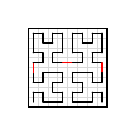
\begin{tikzpicture}
\tikzstyle{helperline} = [lightgray!60!white, line width=0.1mm];
\draw[line cap=round][helperline] (-0.0,0.125) -- (1.0,0.125);
\draw[line cap=round][helperline] (-0.0,0.25) -- (1.0,0.25);
\draw[line cap=round][helperline] (-0.0,0.375) -- (1.0,0.375);
\draw[line cap=round][helperline] (-0.0,0.5) -- (1.0,0.5);
\draw[line cap=round][helperline] (-0.0,0.625) -- (1.0,0.625);
\draw[line cap=round][helperline] (-0.0,0.75) -- (1.0,0.75);
\draw[line cap=round][helperline] (-0.0,0.875) -- (1.0,0.875);
\draw[line cap=round][helperline]  (0.125,1.0) -- (0.125,-0.0);
\draw[line cap=round][helperline]  (0.25,1.0) -- (0.25,-0.0);
\draw[line cap=round][helperline]  (0.375,1.0) -- (0.375,-0.0);
\draw[line cap=round][helperline]  (0.5,1.0) -- (0.5,-0.0);
\draw[line cap=round][helperline]  (0.625,1.0) -- (0.625,-0.0);
\draw[line cap=round][helperline]  (0.75,1.0) -- (0.75,-0.0);
\draw[line cap=round][helperline]  (0.875,1.0) -- (0.875,-0.0);
\draw[line cap=round]  (0,1) rectangle (1,0);
\draw[line cap=round] (0.0625, 0.0625) -- (0.0625, 0.1875);
\draw[line cap=round] (0.0625, 0.1875) -- (0.1875, 0.1875);
\draw[line cap=round] (0.1875, 0.1875) -- (0.1875, 0.0625);
\draw[line cap=round] (0.1875, 0.0625) -- (0.3125, 0.0625);
\draw[line cap=round] (0.3125, 0.0625) -- (0.4375, 0.0625);
\draw[line cap=round] (0.4375, 0.0625) -- (0.4375, 0.1875);
\draw[line cap=round] (0.4375, 0.1875) -- (0.3125, 0.1875);
\draw[line cap=round] (0.3125, 0.1875) -- (0.3125, 0.3125);
\draw[line cap=round] (0.3125, 0.3125) -- (0.4375, 0.3125);
\draw[line cap=round] (0.4375, 0.3125) -- (0.4375, 0.4375);
\draw[line cap=round] (0.4375, 0.4375) -- (0.3125, 0.4375);
\draw[line cap=round] (0.3125, 0.4375) -- (0.1875, 0.4375);
\draw[line cap=round] (0.1875, 0.4375) -- (0.1875, 0.3125);
\draw[line cap=round] (0.1875, 0.3125) -- (0.0625, 0.3125);
\draw[line cap=round] (0.0625, 0.3125) -- (0.0625, 0.4375);
\draw[line cap=round,red] (0.0625, 0.4375) -- (0.0625, 0.5625);
\draw[line cap=round] (0.0625, 0.5625) -- (0.1875, 0.5625);
\draw[line cap=round] (0.1875, 0.5625) -- (0.1875, 0.6875);
\draw[line cap=round] (0.1875, 0.6875) -- (0.0625, 0.6875);
\draw[line cap=round] (0.0625, 0.6875) -- (0.0625, 0.8125);
\draw[line cap=round] (0.0625, 0.8125) -- (0.0625, 0.9375);
\draw[line cap=round] (0.0625, 0.9375) -- (0.1875, 0.9375);
\draw[line cap=round] (0.1875, 0.9375) -- (0.1875, 0.8125);
\draw[line cap=round] (0.1875, 0.8125) -- (0.3125, 0.8125);
\draw[line cap=round] (0.3125, 0.8125) -- (0.3125, 0.9375);
\draw[line cap=round] (0.3125, 0.9375) -- (0.4375, 0.9375);
\draw[line cap=round] (0.4375, 0.9375) -- (0.4375, 0.8125);
\draw[line cap=round] (0.4375, 0.8125) -- (0.4375, 0.6875);
\draw[line cap=round] (0.4375, 0.6875) -- (0.3125, 0.6875);
\draw[line cap=round] (0.3125, 0.6875) -- (0.3125, 0.5625);
\draw[line cap=round] (0.3125, 0.5625) -- (0.4375, 0.5625);
\draw[line cap=round,red] (0.4375, 0.5625) -- (0.5625, 0.5625);
\draw[line cap=round] (0.5625, 0.5625) -- (0.6875, 0.5625);
\draw[line cap=round] (0.6875, 0.5625) -- (0.6875, 0.6875);
\draw[line cap=round] (0.6875, 0.6875) -- (0.5625, 0.6875);
\draw[line cap=round] (0.5625, 0.6875) -- (0.5625, 0.8125);
\draw[line cap=round] (0.5625, 0.8125) -- (0.5625, 0.9375);
\draw[line cap=round] (0.5625, 0.9375) -- (0.6875, 0.9375);
\draw[line cap=round] (0.6875, 0.9375) -- (0.6875, 0.8125);
\draw[line cap=round] (0.6875, 0.8125) -- (0.8125, 0.8125);
\draw[line cap=round] (0.8125, 0.8125) -- (0.8125, 0.9375);
\draw[line cap=round] (0.8125, 0.9375) -- (0.9375, 0.9375);
\draw[line cap=round] (0.9375, 0.9375) -- (0.9375, 0.8125);
\draw[line cap=round] (0.9375, 0.8125) -- (0.9375, 0.6875);
\draw[line cap=round] (0.9375, 0.6875) -- (0.8125, 0.6875);
\draw[line cap=round] (0.8125, 0.6875) -- (0.8125, 0.5625);
\draw[line cap=round] (0.8125, 0.5625) -- (0.9375, 0.5625);
\draw[line cap=round,red] (0.9375, 0.5625) -- (0.9375, 0.4375);
\draw[line cap=round] (0.9375, 0.4375) -- (0.9375, 0.3125);
\draw[line cap=round] (0.9375, 0.3125) -- (0.8125, 0.3125);
\draw[line cap=round] (0.8125, 0.3125) -- (0.8125, 0.4375);
\draw[line cap=round] (0.8125, 0.4375) -- (0.6875, 0.4375);
\draw[line cap=round] (0.6875, 0.4375) -- (0.5625, 0.4375);
\draw[line cap=round] (0.5625, 0.4375) -- (0.5625, 0.3125);
\draw[line cap=round] (0.5625, 0.3125) -- (0.6875, 0.3125);
\draw[line cap=round] (0.6875, 0.3125) -- (0.6875, 0.1875);
\draw[line cap=round] (0.6875, 0.1875) -- (0.5625, 0.1875);
\draw[line cap=round] (0.5625, 0.1875) -- (0.5625, 0.0625);
\draw[line cap=round] (0.5625, 0.0625) -- (0.6875, 0.0625);
\draw[line cap=round] (0.6875, 0.0625) -- (0.8125, 0.0625);
\draw[line cap=round] (0.8125, 0.0625) -- (0.8125, 0.1875);
\draw[line cap=round] (0.8125, 0.1875) -- (0.9375, 0.1875);
\draw[line cap=round] (0.9375, 0.1875) -- (0.9375, 0.0625);
\end{tikzpicture}
\end{document}


\section{\proposedsystem Design and Policies }
\label{sec:design}
Motivated by our findings from the mesoscale carbon analysis, we introduce a carbon-aware framework for edge computing, named \proposedsystem, which employs the variations of carbon intensity across edge data centers to intelligently distribute edge applications while satisfying the low-latency demands. We formalize our carbon-aware edge placement problem with latency constraints and present an optimization approach to minimize carbon emissions at the edge. Lastly, we present our incremental placement algorithm to our edge placement optimization in a real-world edge system. 

% to allocate latency-sensitive edge applications across geographically dispersed edge data centers. Within the system, we introduce a new carbon-aware placement policy aimed at minimizing the carbon footprint of complex edge networks that are composed of \emph{diverse} edge applications and \emph{heterogeneous} edge devices. Lastly, we present the implementation of our system. 

% This section first presents an architectural overview of our \proposedsystem system for carbon-aware edge placement. We then formalize our carbon-aware edge placement problem with latency constraints and present an optimization approach to leverage mesoscale spatial carbon intensity variations to implement carbon-aware placement while considering their applications' tight latency requirements. Lastly, we present our \proposedsystem incremental placement algorithm to our edge placement optimization in a real-world edge system. 

\subsection{\proposedsystem Overview}

\proposedsystem is a carbon-aware framework designed to reduce carbon footprint at the edge by spatially distributing workloads across edge data centers. It manages edge data centers dispersed at mesoscales, which have shown prevalently significant variations in carbon intensity (\autoref{sec:carbon_analysis}), and assumes that edge workloads can shift across edge data centers at this scale. 
Edge servers are not only diverse in geolocations but also diverse in architecture and capacity, exhibiting significant differences in energy efficiency. As carbon emission is a function of energy consumption and carbon intensity of the grid, we further combine intensity variations across edge data center locations and energy efficiency differences across diverse edge servers to save carbon emissions at the edge. As a result,  \proposedsystem reduces edge carbon emissions by placing edge applications on energy-efficient edge servers with sustainable energy supply, respecting the low-latency and resource demands. Moreover, \proposedsystem manages the power states of edge servers to reduce emissions from idle servers. 

\autoref{fig:system_design} shows an overview of our system. The telemetry and carbon intensity services continuously collect system metrics, energy consumption, and the electricity carbon intensity of edge data centers. In addition, the carbon intensity service periodically predicts the carbon intensity of all data centers (step \Circled[inner color=black]{\textbf{0}}). When edge workloads arrive, which can be applications offloaded from resource-limited IoT or mobile devices or applications to be redeployed when an edge server fails (step \Circled[inner color=black]{\textbf{1}}), the placement service instantly decides where to allocate the workloads using a carbon-aware placement policy (step \Circled[inner color=black]{\textbf{2}}). Once the placement decisions are made, the edge orchestrator deploys the applications accordingly (step \Circled[inner color=black]{\textbf{3}}) and establishes the connections to end users (step \Circled[inner color=black]{\textbf{4}}). 

%Next, we introduce the four key components of \proposedsystem. 


% \noindent \textbf{Telemetry.} This component collects static (e.g., location and IP address) and real-time metrics from edge data centers.  The static metrics are used to measure the latency, and the real-time metrics are used to present the system states (e.g., uptime and resource utilization), energy consumption, and hosting applications. 
% % In particular, it gathers the base power consumption when an edge server is idle. 

% % collects the metadata (e.g., location) and real-time resource states, including computing, storage, and network utilization and energy consumption, of edge data centers. The locations can be used to compute latency between edge data centers


% \noindent \textbf{Carbon Intensity Service.} It collects real-time carbon intensity data of all edge data centers based on their locations. Since carbon intensity varies over time, the future carbon intensity would affect the emissions of deployed applications. Therefore, this component provides the forecast carbon intensity of edge data centers using predictive models such as Carboncast~\cite{carboncast}. 


% \noindent \textbf{Placement Service.} This component determines workload placements at runtime. When one or multiple placement requests arrive, it leverages the system's real-time metrics, uptime, and energy consumption profiles and forecasts carbon intensity values to make the placement decisions. We assume each edge workload includes its source location or IP address used for latency measurement, latency SLOs, and application profiles, which indicate the application's resource demands and energy consumption. The application profiles can be obtained by profiling the applications on edge servers or by existing estimation methods~\cite{xxx}. With the above inputs from application and edge data centers, the placement service applies a carbon-aware placement optimization to determine the optimal placements and server activation. 


% \noindent \textbf{Edge Orchestrator.} This component implements the placement decision by deploying applications and activating edge servers accordingly. After deployment, it manages the power states of edge servers and the performance of the active applications. For instance, the edge orchestrator automatically powers off the idle servers to reduce emissions. If an edge server fails, it triggers the replacement of affected applications; if an application becomes overloaded, it scales the replicas and initiates the placement of those replicas. 


% Overall,  \proposedsystem consists of four key components, as illustrated in \autoref{fig:system_design}. 1) \emph{Carbon Intensity Service} provides real-time and forecast carbon intensity values for edge data centers. Edge data centers powered by different energy sources typically exhibit varying carbon intensity values, and forecasted carbon intensity can be obtained using prediction models like Carboncast~\cite{carboncast}; 2) \emph{Telemetry Service} collects the metadata (e.g., location) and real-time resource states, including computing, storage, and network utilization and energy consumption, of edge data centers. The locations can be used to compute latency between edge data centers; 3) \emph{Placement Service} acts as the entry point for application placement. It retrieves the configuration of applications and edge data centers and utilizes the carbon-aware placement policy (described in~\autoref{sec:design_problem}) to determine where to allocate the applications; 4) \emph{Edge Orchestrator} implements the placement decisions and deploys applications on edge data centers. 


% Here, we take edge offloading, where resource-limited IoT devices offload computing-intensive and latency-sensitive applications to edge data centers, as an example to illustrate the carbon-aware edge placement with \proposedsystem. 

% \noindent \textbf{Exemplar Workflow (~\autoref{fig:system_design}).}
% When \proposedsystem is deployed to manage a set of edge data centers, it creates metadata, continuously collects real-time carbon intensity data and system metrics, and predicts the carbon intensity for all edge data centers, shown as step \Circled[inner color=black]{\textbf{0}}. In step \Circled[inner color=black]{\textbf{1}}, IoT devices issue edge application offloading requests to \proposedsystem.  These requests include latency limits, originating locations, and application profiles. In step \Circled[inner color=black]{\textbf{2}}, the Placement Service incorporates configurations of applications and edge data centers and determines the placements using the carbon-aware policy. Among the three edge data centers in~\autoref{fig:system_design}, Edge DC II, which is powered by the most sustainable energy sources (such as solar and wind), is selected to deploy the applications. Once the placements are decided, in step \Circled[inner color=black]{\textbf{3}}, the Edge Orchestrator deploys the applications on Edge DC II and informs the IoT devices of the destinated edge data center, where in step \Circled[inner color=black]{\textbf{4}}, the IoT devices connect and send requests to the offloading applications. 



% We design \proposedsystem by following principles:  

% 1) Geographically dispersed and ephemeral edge resources

% 2) Limited computing, storage, and networking resources

% 3) Heterogeneous edge resources / size and resource types

% 4) Diverse edge applications exhibit different resource requirements

% 5) Latency-critical application. Data residency/sovereignty
 
% Edge data centers are decentralized and near end users. They have limited resources like computing and storage, ranging from a single server rack to a micro data center, exhibiting varied capacity and resource types. Additionally, they often feature transient nodes, with devices frequently joining and leaving the network. Meanwhile, edge applications can exhibit diverse behaviors and resource requirements that defy simple characteristics. 




% ~\autoref{fig:system_design} illustrates our realistic workflow of an edge application and how \proposedsystem augments the placement decisions with carbon-awareness. The workflow starts when a new application placement request arrives 
% in the system \Circled[inner color=black]{\textbf{1}}. The request includes latency limits and the originating location. 
% %Application placement requests can be triggered when a new application arrives or clients increase their latency requirements or request rate.
% In step \Circled[inner color=black]{\textbf{2}}, \proposedsystem utilizes the \autoref{alg:algorithm}, where \proposedsystem will map the edge application to the edge data center with the greenest energy source.
% Lastly, once the placements are decided, in step \Circled[inner color=black]{\textbf{3}}, the Edge Orchestrator implements the placement decisions and informs the client of the destination edge data center, where in step \Circled[inner color=black]{\textbf{4}}, the client connects and send its offloading requests.




% \autoref{fig:system_design} depicts the four key components of \proposedsystem for carbon-aware edge placement between a set of edge data centers.
% \proposedsystem utilizes a \emph{Carbon Intensity Service} that provides real-time and forecast across the edge data center, a \emph{ Telemetry Service}, which collects real-time performance and computes applications' profiles. Moreover, \proposedsystem implements a \emph{Placement Service} that encompasses the carbon-aware placement and power management decisions across different edge data centers while ensuring that resource and performance constraints are strictly met. Lastly, \proposedsystem requires an \emph{Orchestrator Service} (e.g., Kubernetes~\cite{kubernetes}) that implements its placement and power management decisions and establishes the connection between the client and servers. In ~\autoref{sec:implementation}, we discuss these components in more detail. 

\begin{figure}[t]
    \centering
    %\includegraphics[width=0.6\linewidth]{figures/Design.pdf}
    %\includegraphics[width=0.8\linewidth]{figures/carbonedge_design.pdf}
    % \vspace{-6mm}
    \includegraphics[width=1.0\linewidth]{figures/carbonedge_design_walid.drawio.pdf}
    \caption{\proposedsystem design and exemplar workflow of placing offloading applications from IoT devices.}
    \label{fig:system_design}
\end{figure}


\subsection{Carbon-aware Edge Placement}
\label{sec:design_problem}

The section presents the carbon-aware placement with latency constraints problem.  and our proposed policy used in \proposedsystem. Our carbon-aware policy minimizes the carbon footprint of edge data centers using an incremental optimization-driven approach. Our approach holistically integrates three factors: 1) carbon intensity variations of mesoscale edge data centers, 2) workload and diversity in energy efficiency across heterogeneous edge servers, and 3) base power usage and power proportionality of servers.
%of resource  1) energy proportionality of edge applications on heterogeneous edge servers, 2) carbon intensity variations of mesoscale edge data centers, and 3) base load emissions from diverse edge servers to jointly optimize placements at the edge. 

% employs carbon intensity variations across mesoscale edge data centers. This policy solves an integer linear programming (ILP) problem to identify application placements that minimize the carbon footprint of edge data centers, accounting for application diversity and hardware heterogeneity. 



\noindent \textbf{Incremental carbon-aware placement.} Our carbon-aware placement problem aims to minimize carbon emissions from incrementally placing arriving edge applications across edge data centers while meeting strict latency requirements. Given the current power state of the servers $y_j^{curr}: j\in \mathcal{S}$ and available resource capacity $C_j^k$, our objective is to place a batch of applications $\mathcal{A}$ on $\mathcal{S}$.
First, we define two decision variables that represent the placement and power management decisions and then define the carbon emissions associated with the placements based on these two variables. Finally, we present the carbon-aware placement problem formulation. ~\autoref{tab:notations} summarizes the notations. 

\textit{Decision variables:} Let $x_{ij} \in \{0, 1\}$ the placement of application $i \in \mathcal{A}$ on server $j \in \mathcal{S}$, and $y_j \in \{0, 1\}$ indicate whether server $j$ is powered on. These variables are subject to the following four constraint classes.

%%%%%%%%%%%%%%%%%%%%%%%%%%%%%%%%%%%%%%
%%% Table of notations
%%%%%%%%%%%%%%%%%%%%%%%%%%%%%%%%%%%%%%
% Please add the following required packages to your document preamble:
% \usepackage{graphicx}
\begin{table}[tb]
\caption{Notations used in \proposedsystem.}
\label{tab:notations}
\resizebox{.95\linewidth}{!}{%
\begin{tabular}{cl}
% \toprule
\toprule
% \textbf{Decision Variables} &  \\ %\midrule
\multicolumn{2}{l}{\textbf{Decision variables:}} \\ 
$x_{ij} $ & True if application $i$ is placed on server $j$; False otherwise. \\ %\midrule
$y_j $ & True if server $j$ is {\em powered-on}; False otherwise. \\ %\bottomrule %\toprule

\multicolumn{2}{l}{\textbf{Inputs:}}\\ %\midrule
% $M, N$ &  number of servers in the region and number of applications to place \\ \midrule
$C_j^{k}$ &  Available capacity in server $j$ of type $k$ \\ %\midrule
$\bar{I_j}$ &  Average carbon intensity of server $j$ \\ %\midrule
% $T_j^t$ &  Time span of application's execution\\ \midrule
$B_j$ & Base power usage of server $j$ when it is {\em powered-on} \\ %\midrule
$y_j^{curr}$ & Power state (on or off) of server $j$ before placement optimization \\ %\midrule
$R_{ij}^k$ &  Resource demand of type $k$ of application $i$ when running on server $j$ \\ %\midrule
$E_{ij}$ &  Energy usage of application $i$ when running on server $j$ \\ %\midrule
$L_{ij}$ & Latency between application $i$ and server $j$ \\ %\midrule
$\ell_i$ &  Latency requirement of application $i$ \\ %\bottomrule %\toprule

\multicolumn{2}{l}{\textbf{Optimization goal:}}  \\ %\midrule
$f$ & Total carbon footprint of edge placement \\ \bottomrule %\toprule

% \textbf{Intermediate variables} & \textbf{Definition}  \\ \midrule
% $\mathcal{C}_j^{base}$ & Base power carbon emission of server $s_j$ \\ \midrule 
% $\mathcal{C}_{ij}^{app}$ & Carbon emission of running application $a_i$ on server $s_j$ \\ \bottomrule \bottomrule
\end{tabular}%
}
\end{table}


\noindent 1) \textit{Multi-dimensional resource constraint}:  Edge servers are typically computing, storage, and networking resource-limited and are diverse in capacity and resource types. We define $C_j^k$ represents the available capacity of type $k$ on server $j$. When application $i$ runs the server $j$, its resource demands are $R_{ij}^k$. To ensure the application performance, the aggregated resource demands of applications allocated to a server must not exceed its available resources. 
{\small 
\begin{align}
    \label{eq:comp_cap}
    & \sum_i x_{ij} \cdot R_{ij}^k \leq y_j \cdot C_j^{k}, \quad \quad \quad \quad  \forall j, k 
\end{align}
}

\noindent 2) \textit{Latency constraint}: Each application $i$ comes from a certain geolocation and has a specific latency limit $L_i$. The latency from the application's source to the hosting server $L_{ij}$ must remain below this limit. 
{\small 
\begin{align}
    \label{eq:latency}
    & x_{ij} \cdot L_{ij} \leq \ell_i, \quad \quad \quad \quad \quad \quad \quad \quad \forall i, j 
\end{align}
}

\noindent 3) \textit{Placement constraint}: Each application $i$ is assigned to exactly one server. 
{\small 
\begin{align}
    \label{eq:placement}
    & \sum_j x_{ij} = 1, \quad \quad \quad \quad \quad  \quad \quad \quad \quad \quad \forall i 
\end{align}
}

\noindent 4) \textit{Power state consistency}: An active server cannot be powered off during placement (e.g., to avoid service disruption):
{\small 
\begin{align}
    \label{eq:server_keep_on}
    & y_j^{curr} \leq y_j, \quad \quad \quad \quad  \quad \quad \quad \quad \quad \forall j 
\end{align}
}
where $y_j^{curr}$ is the current power state. Additionally, assignments require active servers:  
{\small 
\begin{align}
    \label{eq:server_on}
    & x_{ij} \leq y_j, \quad \quad \quad \quad \quad  \quad \quad \quad \quad \quad \forall i, j 
\end{align}
}
\textit{Carbon emissions:} Carbon emissions from edge placement are from two main sources: application operation and server activation. Application operational emissions depend on the energy consumption of applications and the carbon intensity of hosting servers, given by $\sum_i \sum_j x_{ij} \cdot E_{ij} \cdot \bar{I_j}$, where $E_{ij}$ is the energy consumption of application $i$ on server $j$, and $\bar{I_j}$ is the average carbon intensity of the hosting server $j$. Note that carbon intensity varies over time depending on the mix of energy sources available in that area. $\bar{I_j}$ represents the average of the forecast carbon intensity values of server $j$. Server activation emissions depend on the base power $B_j$ and the carbon intensity $\bar{I_j}$, represented as $\sum_j (y_j - y_j^{curr}) \cdot B_{j} \cdot \bar{I_j}$, where $(y_j - y_j^{curr})$ represents the newly activated server. The total carbon emissions for placing applications are: 
{\small 
\begin{align}
    %\tag{2.1}
    \label{eq:emission}
    & f =  \underbrace{\sum_i \sum_j x_{ij} \cdot E_{ij} \cdot \bar{I_j}}_{\text{Application operation}} + \underbrace{\sum_j (y_j - y_j^{curr}) \cdot B_j \cdot \bar{I_j}}_{\text{Server activation}}
\end{align}
}

\noindent \textit{Problem formulation:} The carbon-aware placement policy identifies the optimal placement $x_{ij}^*$ and power management $y_j^*$ solutions to minimize carbon emissions at the edge while meeting the latency and resource constraints. The problem is formulated as follows: 

{\small 
\begin{align}
    %\tag{2.1}
    \label{eq:objective}
    & \min_{\substack{x_{ij}^*, y_j^*}}  \quad f  \quad \quad \quad \quad \text{s.t. Constraints 1-5 hold. }
\end{align}
}

% \noindent{\bf Dimensionality reduction.} Edge servers $\mathcal{S}$ are grouped by edge data center locations $\mathcal{L}$, with $S_l$ servers at location $l$. A na\"{\i}ve 3D formulation (application-location-server) requires  $|A| \times |L| \times max(S_l)$ variables. However, server distributions are often skewed (e.g., urban areas have denser deployments), making $\sum_{l \in \mathcal{L}} S_l\ll |L| \times max(S_l)$. By flatting to a 2D model (application-server), we reduce the variable count to $|A| \times S_{total}$, where $S_{totoal} = \sum_{l \in \mathcal{L}} S_l$. For $|A|=100$, $|L|=5$, $max(S_l)=20$, and $|S_{total}|=50$, this cuts variables from 10,000 to 5,000--a 50\% reduction.  Importantly, our model preserves locality: servers retain location-specific attributes (e.g., $I_j$ and $L_{ij}$), so constraints remain semantically unchanged. 

 
\noindent{\bf Extensions.} The above formulation focuses on reducing carbon emissions as a primary goal while considering edge latency as a constraint. Alternatively, a multi-objective optimization can be employed to minimize both carbon emissions and latency. Additionally, other objectives like energy usage can also be optimized alongside carbon in a similar fashion. In ~\autoref{sec:eval_carbon_energy}, we  demonstrate the benefits of such a multi-objective optimization strategy, which navigates the trade-offs between carbon emissions and energy usage in edge computing.

% As discussed in ~\autoref{sec:eval_carbon_energy}, this multi-objective optimization strategy is advantageous for navigating the trade-offs between carbon emissions and energy usage in edge computing.



\begin{algorithm}[t]
\scriptsize
\caption{\proposedsystem Incremental Placement Algorithm}
\label{alg:algorithm}
\raggedright
\textbf{Input:} Arriving applications $\mathcal{A}$,  Servers $\mathcal{S}$, Latency requirements $\boldmath{\ell}$, Resource demands $\mathbf{R}$, and Energy consumption $\mathbf{E}$ \\
\textbf{Output:} Placement ($\mathbf{x}$) and Power ($\mathbf{y}$) decisions.
\begin{algorithmic}[1]
\State Initialize latency matrix $\mathbf{L} \gets \emptyset$
\For{each application $a_i \in \mathcal{A}$}
\For {each server $s_j \in \mathcal{S}$}
\State $\mathbf{L}_{ij} \gets \textsc{CalculateLatency}(a_i, s_j)$ \label{ln:latency_calc} \Comment{Get application-server latency\quad }
% \State $\mathbf{L} \gets \mathbf{L} \cup L_{ij}$
\EndFor
\EndFor

\State $\mathcal{S}', \mathbf{L}' \gets \textsc{FilterFeasibleServers}(\mathcal{A}, \mathcal{S}, \mathbf{L}, \boldmath{\ell})$ \label{ln:preprocess} \Comment{Select servers satisfying latency limits}

\State $\mathbf{C}, B, \bar{I}, \mathbf{y}^{curr} \gets \textsc{GetServerStates}(\mathcal{S}')$ 
\Comment{Available capacities $\mathbf{C}$, base power $B$, mean carbon intensity $\bar{I}$, current power states $\mathbf{y}^{curr}$ }

\State $\mathbf{x}, \mathbf{y} \gets \textsc{SolveOptimization}(\mathcal{A}, \mathcal{S}', \boldmath{\ell}, \mathbf{R}, \mathbf{E}, \mathbf{C}, B, \bar{I} , \mathbf{y}^{curr}, \mathbf{L}')$ \label{ln:solve}
\Comment{Solve \autoref{eq:objective}}

\State $\mathbf{C}' \gets \textsc{UpdateServerStates}(\mathbf{x}, \mathbf{y}, \mathcal{C})$ \label{ln:update}
\Comment{Update servers capacity}  \\

\Return $\mathbf{x}, \mathbf{y}$
\end{algorithmic}
\end{algorithm}


\subsection{\proposedsystem Placement Algorithm}\label{sec:design_algorithm}
Our placement algorithm assumes that latency-sensitive edge applications may arrive unpredictably and need to be placed onto edge data centers in a carbon-aware manner. To achieve this, \proposedsystem employs an incremental placement strategy, executing the algorithm periodically to process newly arriving applications as a batch, to ensure carbon-efficient placement without global recomputation, as shown in \autoref{alg:algorithm}.

The algorithm places a set of arriving applications $\mathcal{A}$ (with latency requirements $\boldmath\ell$, resource demands $\mathbf{R}$, and energy profiles $\mathbf{E}$) across edge servers $\mathcal{S}$ in mesoscale data centers. First, it computes application-server latency $\mathbf{L}$ and prunes (i.e., filters out) servers exceeding latency constraints, retaining only feasible candidates $\mathcal{S}' \in \mathcal{S}$ (line 1-8). Next, it retrieves server telemetry (available capacity $\mathbf{C}$, base power $B$, current power state $y^{curr}$) and  mean carbon intensity $\bar{I}$ (line 9). Then, it solves the optimization in ~\autoref{eq:objective} using the latency-compliant server set $\mathcal{S}'$ to ensure traceability. 
Placing incoming applications in small batches in real-time can be done efficiently---our  result in ~\autoref{sec:eval_overhead} shows that  incremental placement of a batch of 50 newly arriving applications across 400 servers completes in 3 seconds (line 10). Finally, \proposedsystem commits the resource allocation and power state transition, updating server states for the next iteration (line 11).


% periodically and incrementally places all newly arriving applications as a batch as shown in  \autoref{alg:algorithm}. 
%The problem formulation above relies on detailed knowledge of all applications' resource requirements and carbon intensity and assumes all applications are ready upfront. In practice, however, carbon intensity forecasts are only available for a few days, and applications arrive \emph{incrementally}, stay for arbitrary time, and request rates may change with time.
%\autoref{alg:algorithm} illustrates the steps to place a new application or a batch of applications in a carbon-aware manner. 



% The first step is to estimate the resource requirements of each new application by profiling it for $t$ seconds or utilizing a performance model~\cite{paleo,justus2018,cai2017neuralpower, performance_modeling}. After estimating the applications' resource requirements, the placement service utilizes ILP formulation in equations ~\ref{eq:objective}-\ref{eq:binary} while only considering the new applications and the idle resources. Note that, we utilize $\hat{I}_j$ instead of the time-varying carbon intensity $I_j^t$ and to ensure consistency with the current status, we add a constraint $y_j^{curr} \leq y_j \forall j$, which ensures that {\em powered-on} servers remains on. The resource utilization of servers at all edge locations is updated using the computed placement for the next iteration.


% Edge applications exhibit different duration requirements depending on the use cases, such as long-term and short-lived applications. To address these variations, \proposedsystem implements two optimization strategies.

% \noindent{\bf Long-term applications.}
% Applications such as smart city infrastructure monitoring or industrial automation systems demand uninterrupted long-term execution and tolerate gradual deployment optimizations and periodic re-optimization. The Placement Service solves the ILP problem exactly to identify the optimal placement and power management plan. 

% % Note that the computational overhead to solve the ILP does not interfere with application latency requirements, as \proposedsystem operates on a dedicated orchestration server isolated from edge work execution. 

% \noindent{\bf Short-lived applications.} Conversely, short-lived applications (e.g., augmented reality (AR) rendering) require sub-second placement with stringent latency constraints. We use a greedy heuristic to address the time-sensitive placement needs of short-lived applications. The algorithm first filters candidate edge servers that satisfy the application's latency (\autoref{eq:comp_cap}) and resource requirements (\autoref{eq:latency}). Next, for each candidate, it estimates the carbon emissions using the objective function defined in~\autoref{eq:objective} and selects the server yielding the minimum emissions. 
% Additionally, idle servers are automatically powered off post-execution to minimize carbon emissions. 


% \noindent{\bf Applications profiles.} Application profiles, such as resource demands $R_{ij}^k$ and energy consumption $E_{ij}$, are essential for making the placement decisions. These profiles can be obtained by profiling applications on servers or estimating using existing methods~\cite{XXX}. 

% \noindent{\bf Dynamic workloads.} The workloads of edge applications fluctuate over time. To maximize carbon emission reductions without compromising service continuity, \proposedsystem can integrate with the auto-scaler of the Edge Orchestrator, optimizing replica placement and managing workload distribution via the load balancer. 

% \noindent{\bf Temporal carbon intensity.} 
% \noindent{\bf Workload Fluctuation.} 



% \subsection{\proposedsystem Implementation}
% Lastly, we present the implementation of \proposedsystem, built on top of Sinfonia~\cite{satyanarayanan2022sinfonia}, an open-source orchestrator for edge-native applications. Our implementation realizes the \proposedsystem components as follows:

% \noindent\textbf{Carbon Intensity Service}: We built our carbon intensity service by integrating historical traces from Electricity Maps~\cite{electricity-map} and using the traces to provide real-time and forecast carbon intensity.

% \noindent\textbf{Telemetry Service}: \proposedsystem collects real-time performance, resource, and energy consumption telemetry from edge data centers. These telemetries are based on Prometheus monitoring stacks. We augmented Prometheus with power monitoring capabilities. To measure the power consumption of CPU servers using RAPL~\cite{david2010rapl}, while for GPU servers, we leveraged Prometheus's DGCM exporter~\cite{nvidia_dcgm_exporter_github}. 
% Our telemetries are integrated into Sinfonia’s dynamic attributes and updated periodically. Additionally, we include latency data based on round-trip time (RTT) measurements from WonderNetwork. Finally, alongside the telemetries, we implement an application profiling service that gathers application performance metrics, such as latency, power consumption, resource demands, and other crucial information for accurate placement decisions across available resources. 


% \noindent\textbf{Placement Service}: We implement the placement service with Python, and the carbon-aware placement optimization is solved using the Google OR-Tools~\cite{ortools}, an interface to the branch and cut solver. It gets the configuration of applications and edge data centers and outputs the placement and power management decisions to the edge orchestrator. 

% % The \proposedsystem placement service encompasses the carbon-aware placement and power management decisions across different edge data centers. As we detailed in ~\autoref{sec:design_algorithm}, 
% % the placement service integrates its knowledge of the carbon intensity, resource requirements, and load to compute the decisions that optimize the total carbon emissions while ensuring that resource and performance constraints are strictly met. 
% % We implement \autoref{alg:algorithm} using Python and Google OR-Tools~\cite{ortools}. 


% \noindent\textbf{Edge Orchestrator}: We leverage Sinfonia, which is built on top of Kubernetes~\cite{kubernetes}, to deploy and manage server states. After getting the placement decisions, Sinfonia initiates the deployment sequence (Sinfonia RECIPE) to the destination servers or activates servers if necessary and informs the client(s) of the destination's address.  Note that although Sinfonia is packed with fault-tolerance and reconfiguration capabilities, evaluating them is beyond the scope of this paper.

% In addition to the prototype of \proposedsystem, we developed a simulator for large-scale placement evaluations, in which we simulate diverse edge settings with dynamic workloads and heterogeneous servers. This simulator implements the carbon-aware placement policy and other baseline policies using Google OR-Tools~\cite{ortools}. The simulator and the \proposedsystem policies were implemented in Python with approximately 1,000 lines of code.


% The placement policy is to minimize the carbon emissions of edge data centers, including emissions from applications and powered-on servers. The carbon emission of applications are $\sum_{i=1}^N \sum_{j=1}^M x_{ij} \cdot E_{ij} \cdot I_j$, and the emissions from active servers are $\sum_{j=1}^M y_{j} \cdot B_{j} \cdot I_j$, and the total carbon emissions is:

% {\small 
% \begin{align}
%     %\tag{2.1}
%     \label{eq:objective}
%     & C(t) =  \sum_{i=1}^N \sum_{j=1}^M x_{ij} \cdot E_{ij} \cdot I_j^t + \sum_{j=1}^M y_{j} \cdot B_{j} \cdot I_j^t
% \end{align}
% }

% {\small 
% \begin{align}
%     %\tag{2.1}
%     \label{eq:objective}
%     & \text{min} \quad \mathcal{C}^{total} \\
%     &\mathcal{C}^{total} =  \sum_{j=1}^M y_j \cdot  \mathcal{C}_{j}^{base} + \sum_{i=1}^N \sum_{j=1}^M x_{ij} \cdot \mathcal{C}_{ij}^{app} \quad & \nonumber \\
%     &\mathcal{C}_{ij}^{app} = \sum_{t\in T_i} E_{ij} \cdot I_j^t \quad , \quad \mathcal{C}_{j}^{base} = \sum_{t\in T_i} P_j^{base} \cdot I_j^t & \nonumber \\
%     \textbf{s.t.} \quad &  \nonumber \\
%     %\tag{2.2}
%     \label{eq:comp_cap}
%     & \sum_{i=1}^N x_{ij} \cdot R_{ij}^k \leq y_j \cdot \mathcal{R}_j^{k}, \quad \forall j, k \\
%     %\tag{2.3}
%     % \label{eq:band_cap}
%     % & \sum_{i=1}^N x_{ij} \cdot B_{ij} \leq y_j \cdot B_j^{max}, \quad \forall j \\
%     %\tag{2.4}
%     \label{eq:latency}
%     & x_{ij} \cdot L_{ij} \leq L_i, \quad \forall i, \forall j \\
%     %\tag{2.5}
%     \label{eq:placement}
%     & \sum_{j=1}^M x_{ij} = 1, \quad \forall i \\
%     %\tag{2.6}
%     \label{eq:server_on}
%     & x_{ij} \leq y_j, \quad \forall i, \forall j\\
%     %\tag{2.7}
%     \label{eq:binary}
%     & x_{ij}, y_j \in \{0,1\}, \quad \forall i, \forall j
% \end{align}
% }




% We define the carbon-aware placement problem as a minimization problem of the total carbon emissions from active applications and base power from {\em powered-on} servers while satisfying the application's resource and latency requirements.  Further, \proposedsystem formulates this as an integer linear programming (ILP) problem. The variables used in the problem are summarized in Table~\ref{tab:notations}. 

% Two binary decision variables are used: \todo{We just repeated what is in the table.}

% \begin{enumerate}
%     \item $x_{ij} \in \{0, 1\}$, where $x_{ij} = 1$  indicates that application $a_i$ is placed on server $s_j$, and $x_{ij}=0$ otherwise;
%     \item $y_j \in \{0, 1\}$, where $y_j = 1$ indicates that server $s_j$ is {\em powered-on}, and $y_j = 0$ indicates the server is {\em powered-off}.   
% \end{enumerate}

% We formulate the problem as a minimization problem as follows: 

% As shown, \autoref{eq:objective} aims to minimize the total carbon emissions of application execution and base power, where emissions  
% of running application, $a_i$ on server $s_j$ is defined as ${C}_{ij}^{app}$, which considers the energy consumption and the time-varying carbon intensity across different servers, and the carbon emission from base power from {\em powered-on} servers, denotes as $\mathcal{C}_{j}^{base}$.
% \autoref{eq:comp_cap} ensures that the server's various resource capacities are not exceeded, accounting for heterogeneity in server resources. In particular, we utilize three types of resources: utilization, memory, and bandwidth, where we estimate the utilization based on the application's processing time and request rate~\cite{Clockwork}.% following the method described in~\cite{weee21, Clockwork}.
% ~\autoref{eq:latency} enforces that the end-to-end latency from application $a_i$ to server $s_j$ does not exceed the application's allowable latency. \autoref{eq:placement} ensures each application is placed on exactly one server, while \autoref{eq:server_on} guarantees that an application can only be placed on {\em powered-on} servers. Finally, \autoref{eq:binary} ensures that the decision variables are binary.



%Note that although the above only considers carbon emissions in its objectives and considers latency as energy consumption as part of the constraints and by-product of the carbon savings. Augmenting \autoref{eq:objective} with energy or latency objectives and formulating the problem as a multi-objective optimization is beneficial in navigating the carbon-latency and carbon-energy trade-offs, as we will show in ~\autoref{sec:hetero}.

% \begin{algorithm}[t]
% \footnotesize
% \caption{\proposedsystem Algorithm}
% \label{alg:algorithm}
% \raggedright
% \textbf{Input:} New Applications $N$, Latency Requirements $L$, Servers $M$, Power status $y^{curr}$, Available Resources $\mathcal{R}^{idle}$, and Mean Carbon Intensity $\mathcal{\bar{I}}$. \\
% \textbf{Output:} Placement ($x$) and Power ($y$) decisions.
% \begin{algorithmic}[1]
% \State $\hat{R} \gets []$
% \For{$a_i \in N$}
% \For {$s_i \in M$}
% \State $R_{ij}^k \gets$ \text{Profile}$(a_i, s_j)$ \Comment{Profile or estimate resource requirements.\quad \quad \quad \quad \quad \quad \quad \quad \quad \quad \quad }
% \State $\hat{R}.\text{append}(R_{ij})$\
% \EndFor
% \EndFor
% \State $x,y \gets$ Solve Optimization($N, L, M, y^{curr}, \hat{R}, \mathcal{R}^{idle} , \mathcal{\hat{I}}$)\\
% \Return $x,y$
% \end{algorithmic}
% \end{algorithm}


% \begin{algorithm}[t]
% \footnotesize
% \caption{\proposedsystem Algorithm}
% \label{alg:algorithm}
% \raggedright
% \textbf{Input:} New Applications $N$, Latency Requirements $L$, Servers $M$, Power status $y^{curr}$, Available Resources $\mathcal{R}^{idle}$, and Mean Carbon Intensity $\mathcal{\bar{I}}$. \\
% \textbf{Output:} Placement ($x$) and Power ($y$) decisions.
% \begin{algorithmic}[1]
% \State $\hat{R} \gets []$
% \For{$a_i \in N$}
% \For {$s_i \in M$}
% \State $R_{ij}^k \gets$ \text{Profile}$(a_i, s_j)$ \Comment{Profile or estimate resource requirements.\quad \quad \quad \quad \quad \quad \quad \quad \quad \quad \quad }
% \State $\hat{R}.\text{append}(R_{ij})$\
% \EndFor
% \EndFor
% \State $x,y \gets$ Solve Optimization($N, L, M, y^{curr}, \hat{R}, \mathcal{R}^{idle} , \mathcal{\hat{I}}$)\\
% \Return $x,y$
% \end{algorithmic}
% \end{algorithm}





% \subsection{Online Placement Algorithms}\label{sec:design_algorithm}
% Our edge placement algorithm assumes that new applications can arrive into the system at any time and need to be placed onto edge data centers in a carbon-aware manner while meeting their latency constraints. To do so, we assume that the algorithm runs periodically and incrementally places all newly arriving applications as a batch as shown in  \autoref{alg:algorithm}. 
% %The problem formulation above relies on detailed knowledge of all applications' resource requirements and carbon intensity and assumes all applications are ready upfront. In practice, however, carbon intensity forecasts are only available for a few days, and applications arrive \emph{incrementally}, stay for arbitrary time, and request rates may change with time.
% %\autoref{alg:algorithm} illustrates the steps to place a new application or a batch of applications in a carbon-aware manner. 
% As shown, the algorithm takes the set of new applications $N$, their latency requirements, the set of servers $M$, their power status $y^{curr}$, available resource $\mathcal{R}^{idle}$, and a per-location forecast of mean carbon intensity $\bar{I}$. The first step is to estimate the resource requirements of each new application by profiling it for $t$ seconds or utilizing a performance model~\cite{paleo,justus2018,cai2017neuralpower, performance_modeling}. After estimating the applications' resource requirements, the placement service utilizes ILP formulation in equations ~\ref{eq:objective}-\ref{eq:binary} while only considering the new applications and the idle resources. Note that, we utilize $\hat{I}_j$ instead of the time-varying carbon intensity $I_j^t$ and to ensure consistency with the current status, we add a constraint $y_j^{curr} \leq y_j \forall j$, which ensures that {\em powered-on} servers remains on. The resource utilization of servers at all edge locations is updated using the computed placement for the next iteration.

% \begin{align}
%     %\tag{2.1}
%     \label{eq:objective_alg}
%     & \text{min} \quad \mathcal{C}^{total} =  \sum_{j=1}^M y_j \cdot  \mathcal{C}_{j}^{base} + \sum_{i=1}^N \sum_{j=1}^M x_{ij} \cdot \mathcal{C}_{ij}^{app} \quad & \\
%     &\mathcal{C}_{ij}^{app} = E_{ij} \cdot \bar{I_j} \quad , \quad \mathcal{C}_{j}^{base} =  P_j^{base} \cdot \bar{I_j} & \nonumber \\
%     \textbf{s.t.} \quad &  \nonumber \\
%     %\tag{2.2}
%     \label{eq:comp_cap_alg}
%     & \sum_{i=1}^N x_{ij} \cdot R_{ij}^k \leq y_j \cdot \mathcal{R}_j^{k}, \quad \forall j, k \\
%     %\tag{2.3}
%     % \label{eq:band_cap}
%     % & \sum_{i=1}^N x_{ij} \cdot B_{ij} \leq y_j \cdot B_j^{max}, \quad \forall j \\
%     %\tag{2.4}
%     \label{eq:latency_alg}
%     & x_{ij} \cdot L_{ij} \leq L_i, \quad \forall i, \forall j \\
%     %\tag{2.5}
%     \label{eq:placement_alg}
%     & \sum_{j=1}^M x_{ij} = 1, \quad \forall i \\
%     %\tag{2.6}
%     \label{eq:server_on_alg}
%     & x_{ij} \leq y_j, \quad \forall i, \forall j\\
%     %\tag{2.7}
%     \label{eq:binary_alg}
%     & x_{ij}, y_j \in \{0,1\}, \quad \forall i, \forall j
% \end{align}



% Given an edge network, it includes geographically dispersed edge data centers containing a total of $M$ servers, represented as $S = \{s_1, s_2, ..., s_M\}$. Each server $s_j$ is equipped with various resources--such as CPU, Memory, and Bandwidth--where $C_j^k$ indicates the maximum available resources of type $k$ on server $j$. Furthermore, each {
% \em powered-on} server has a base power consumption denoted by $B_j$. Every server $s_j$ resides in an edge data center and is powered by an energy source that has a carbon intensity value, $I_j$, which is time-varying according to the mix of energy sources available in that area.

% Let us consider, at time $t$,  $N$ application placement requests arrive,  represented as $A = \{a_1, a_2, ..., a_N\}$. These placement requests can be from various locations, and each application $a_i$ comes with specific latency requirements $L_i$, alongside energy consumption and resource needs. These energy consumption rates and resource requirements differ depending on the edge servers hosting them (refer to ~\autoref{fig:models_profile}). When an application $a_i$ is executed on the server $s_j$, its resource demand is indicated as $R_{ij}^k$, while the energy consumption is represented as $E_{ij}$. Additionally, the end-to-end latency connecting the workload of application $a_i$ to server $s_j$ is denoted by $L_{ij}$.

% We define two decision variables. Let $x_{ij} \in \{0, 1\}$ indicate the application placement decision, where $x_{ij} = 1$ means that application $a_i$ is placed on server $s_j$, and $x_{ij} = 0$ otherwise. Let $y_j \in \{0, 1\}$ indicate the server power status, where $y_j = 1$ indicates that server $s_j$ is turned on, and $y_j = 0$ indicates that the server is off. 

% These variants need to meet four constraints. First, the request demands cannot exceed the resource capacity of powered-on servers (\autoref{eq:comp_cap}). Second, the placements need to meet latency limits (\autoref{eq:latency}). Third, all applications need to be placed on a server (\autoref{eq:placement}). Fourth, applications can only be placed on powered-on servers (\autoref{eq:server_on}). Fifth, a powered-on server cannot be powered off. We formulate the four constraints as follows.

% {\small 
% \begin{align}
%     \label{eq:comp_cap}
%     & \sum_{i=1}^N x_{ij} \cdot R_{ij}^k \leq y_j \cdot C_j^{k}, \quad \quad \quad \quad  \forall j, k \\
%     %\tag{2.4}
%     \label{eq:latency}
%     & x_{ij} \cdot L_{ij} \leq L_i, \quad \quad \quad \quad \quad \quad \quad \quad \forall i, j \\
%     %\tag{2.5}
%     \label{eq:placement}
%     & \sum_{j=1}^M x_{ij} = 1, \quad \quad \quad \quad \quad  \quad \quad \quad \quad \quad \forall i \\
%     %\tag{2.6}
%     \label{eq:server_on}
%     & x_{ij} \leq y_j, \quad \quad \quad \quad \quad  \quad \quad \quad \quad \quad \forall i, j \\
%     \label{eq:server_keep_on}
%     & y_j^{curr} \leq y_j, \quad \quad \quad \quad \quad  \quad \quad \quad \quad \quad \forall j
% \end{align}
% }


\section{\proposedsystem Implementation}
\label{sec:implementation}
This section describes the implementation of \proposedsystem (See ~\autoref{fig:system_design}) on top of Sinfonia~\cite{satyanarayanan2022sinfonia}, a Kubernetes based open-source orchestrator for edge-native applications. Our implementation adds $\sim$4k SLOC to the  Sinfonia system and is available as open source \emph{(URL blinded)}. 
%Lastly, we describe our simulation environment used in large-scale experiments.

\subsection{\proposedsystem Prototype}
\noindent Our \proposedsystem consists of the following components that we added to Sinfonia.

\noindent\textbf{Telemetry Service}:
Our telemetry service is integrated into Sinfonia’s telemetry, where it collects static (e.g., location and IP address) attributes and real-time  (e.g., utilization) metrics. Real-time metrics are collected based on Prometheus monitoring stack\cite{Prometheus}. We augment Sinfonia's monitoring with the following metrics:
\begin{enumerate}[leftmargin=*]
    \item \textbf{Power Monitoring}: We measure the power consumption of CPU servers using RAPL~\cite{david2010rapl}, and we leveraged Prometheus's DGCM exporter for GPUs~\cite{nvidia_dcgm_exporter_github}. 

    \item \textbf{Carbon Intensity}: We integrate a carbon intensity service that replays historical traces from Electricity Maps~\cite{electricity-map} and uses the traces to provide real-time and forecast carbon intensity.

    \item \textbf{Carbon Monitoring}: We implement carbon monitoring based on energy usage and the carbon intensity of the selected edge sites, where we account for the base power (if the server is turned on) and applications energy usage. 
    
    \item \textbf{End-to-end latency}: In addition to latency across sites, we recorded end-to-end latency between users and their deployed applications.

\end{enumerate}

\noindent\textbf{Profiling Service}: 
We implement an application profiling service that collects the application's performance metrics, such as latency, power consumption, resource demands, and other crucial information, to make accurate placement decisions across available resources. Our profiling service can be replaced with performance models that statically analyze the applications and predict the latency and energy consumption~\cite{paleo, cai2017neuralpower}.

\noindent\textbf{Placement Service}:
Lastly, we implement our placement policy (\autoref{alg:algorithm}) on sinfonia as a matching policy. The placement policy utilizes the system's real-time metrics, static attributes of different edge sites, and workload profiles to determine optimal placements and server activation.
Our implementation batches deployment requests (e.g., every 5 minutes) and solves the optimization problem per application batch using the Google OR-Tools~\cite{ortools}. We demonstrate the effectiveness of our approach in ~\autoref{sec:eval_overhead}. 
%, an interface to the branch and cut solver.
%It gets the configuration of applications and edge data centers and outputs the placement and power management decisions to the edge orchestrator. 
%\noindent\textbf{Edge Orchestrator}: 
%The placement decision are then utilized by the orchestrations service that 
%We leverage Sinfonia, which is built on top of Kubernetes~\cite{kubernetes}, to deploy and manage server states. 
After computing the placement decisions, we utilize Sinfonia's orchestration capabilities to initiate the deployment sequence (Sinfonia RECIPE), which contains the necessary Kubernetes deployment files and helm charts, to the destination servers or activate servers if necessary and inform the client(s) of the destination's address. Note that although Sinfonia and our system are packed with fault-tolerance and reconfiguration capabilities, evaluating them is beyond the scope of this paper.







% \noindent\textbf{Telemetry Service}: \proposedsystem collects real-time performance, resource, and energy consumption telemetry from edge data centers. These telemetries are based on Prometheus monitoring stacks\cite{Prometheus}. We augmented Prometheus with power monitoring capabilities, where we measure the power consumption of CPU servers using RAPL~\cite{david2010rapl}, and for GPU servers, we leveraged Prometheus's DGCM exporter~\cite{nvidia_dcgm_exporter_github}. 
% Our telemetries are integrated into Sinfonia’s dynamic attributes and updated periodically. Lastly, we record end-to-end latency between users and their applications.

% \noindent\textbf{Carbon Intensity Service}: We built our carbon intensity service by integrating historical traces from Electricity Maps~\cite{electricity-map} and using the traces to provide real-time and forecast carbon intensity.


%Additionally, we include latency data based on round-trip time (RTT) measurements from WonderNetwork. Finally, alongside the telemetries, we implement an application profiling service that gathers application performance metrics, such as latency, power consumption, resource demands, and other crucial information for accurate placement decisions across available resources. 


% \noindent\textbf{Placement Service}: We implement the placement service with Python, and the carbon-aware placement optimization is solved using the Google OR-Tools~\cite{ortools}, an interface to the branch and cut solver. It gets the configuration of applications and edge data centers and outputs the placement and power management decisions to the edge orchestrator. 

% The \proposedsystem placement service encompasses the carbon-aware placement and power management decisions across different edge data centers. As we detailed in ~\autoref{sec:design_algorithm}, 
% the placement service integrates its knowledge of the carbon intensity, resource requirements, and load to compute the decisions that optimize the total carbon emissions while ensuring that resource and performance constraints are strictly met. 
% We implement \autoref{alg:algorithm} using Python and Google OR-Tools~\cite{ortools}. 


% \noindent\textbf{Edge Orchestrator}: We leverage Sinfonia, which is built on top of Kubernetes~\cite{kubernetes}, to deploy and manage server states. After getting the placement decisions, Sinfonia initiates the deployment sequence (Sinfonia RECIPE) to the destination servers or activates servers if necessary and informs the client(s) of the destination's address.  Note that although Sinfonia is packed with fault-tolerance and reconfiguration capabilities, evaluating them is beyond the scope of this paper.

\subsection{\proposedsystem Edge Simulator}
In addition to the prototype of \proposedsystem, we developed a simulator for larger-scale evaluations 
that is not feasible using an edge testbed.
Our simulator supports
simulating diverse edge settings with dynamic workloads and heterogeneous servers. This simulator represents the components of Sinfonia and follows the same decision process and metrics, where we implement our proposed carbon-aware placement policy and other baseline policies using Google OR-Tools~\cite{ortools}. The \proposedsystem simulator is implemented in Python using $\sim$2k SLOC.

%Sinfonia consists of three tiers: Tier 1, the cloud; Tier 2, edge sites; and Tier 3, end devices. Tiers 1 and 2 are Kubernetes clusters (K3s) equipped with Prometheus-based monitoring stacks. Tier 1 serves as the control plane, receiving offloading (placement) requests from Tier 3, selecting appropriate edge sites in Tier 2,  and responding with placement decisions. It maintains a CloudletTable that stores both static (e.g., location) and dynamic (e.g., resource utilization) attributes of Tier 2 servers, allowing for placement decisions based on predefined matches (policies). Sinfonia's flexibility to support customer matches allowed us to seamlessly integrate \proposedsystem's carbon-aware placement policy. 

% We built our Carbon Intensity Service (see ~\autoref{sec:design_arch}) by integrating historical traces from Electricity Maps~\cite{electricity-map} and using the traces to provide real-time and forecasted carbon intensity for edge servers in Tier 2. We map each edge data center to a carbon zone by utilizing its geographic coordinates. 





% In addition, we augmented the telemetries in Sinfonia (e.g., utilization, response time) with power monitoring capabilities. To measure power consumption of CPU servers using RAPL~\cite{david2010rapl}, while for GPU servers, we leveraged Prometheus's DGCM exporter~\cite{nvidia_dcgm_exporter_github}. These energy metrics, along with the carbon intensity data, were integrated into Sinfonia’s dynamic attributes and periodically updated from Tier 2 to Tier 1 (default interval of 15 seconds). All dynamic metrics are stored in the CloudletTable in Tier 1 for informed placement decision-making. To include the latency data, we utilized the round-trip time (RTT) measurements from WonderNetwork, stored in a configuration file.

% We implemented \autoref{alg:algorithm} as a new \emph{matcher} in Sinfonia's Tier 1. When a new application arrives (i.e., a Sinfonia RECIPE), the matcher batches applications, utilizes the available resources and solves the ILP using Google OR-Tools~\cite{ortools}. After mapping the application to servers,  Sinfonia initiates the deployment sequence and informs the client(s) (Tier 3) of the destination's address. Note that, although Sinfonia is packed with fault-tolerance and reconfiguration capabilities, evaluating them are beyond the scope of this paper. 





%\clearpage
\section{Evaluation}
\label{sec:evaluation}

In this section, we evaluate the performance of \proposedsystem using real experiments and large-scale simulations. We start with evaluating \proposedsystem in mesoscale edge deployments, showcasing its efficiency in reducing carbon emissions on a regional scale. Next, we extend our analysis to continental-scale edge data centers (e.g., a Content Delivery Network, CDN), highlighting that the benefits of saving carbon emissions with granular carbon intensity are commonplace. In doing so, we address the following questions:

\begin{enumerate}[leftmargin=*]
    \item {\em What are the potential carbon savings of spatial shifting for an edge provider with multiple regional edge data center locations?}
    \item {\em How can a CDN exploit mesoscale variations for carbon-aware edge hosting across a large network of edge locations? How do latency limits affect potential carbon savings?}
    \item {\em How do seasonal variations, demand, and capacity affect carbon savings and placement decisions?}
    \item {\em How does the heterogeneity in edge resources impact savings? What are the carbon-energy trade-offs in these settings?}
\end{enumerate}

Next, we detail our real-world datasets, experimental settings, baselines, and evaluation metrics.

\begin{figure}[t]
    \centering
    \includegraphics[width=0.6\linewidth]{figures/7_energy_consumption_models_legend.pdf}\\
    \subfloat[\centering Energy]{\includegraphics[width=0.3\linewidth]{figures/7_energy_consumption_models.pdf}%
    \label{fig:models_profile_energy}%
    }%
    % \quad
    % \subfloat[\centering SLO-App]{
    % \includegraphics[width=0.22\linewidth]{figures/ru_gpu_mem_latency.pdf}
    % \label{fig:comparion_regions_real_latency}
    % }%
    % \quad
    \subfloat[\centering GPU Memory]{
    \includegraphics[width=0.3\linewidth]{figures/7_gpu_memory_models.pdf}
    \label{fig:models_profile_memory}
    }%
    % \quad
    \subfloat[\centering Inference Time]{
    \includegraphics[width=0.3\linewidth]{figures/7_inference_time_models.pdf}
    \label{fig:models_profile_latency}
    }%
    \caption{Energy consumption, memory usage, and inference time of ML workloads across devices.}
    \label{fig:models_profile}
\end{figure}

\subsection{Experimental Methodology}
\subsubsection{Real World Traces.}\label{sec:real_world_traces}\hfill\\
This section describes our real-world traces and how we combined them in our evaluations.

\noindent{\bf Carbon Intensity Traces.}
We utilize the carbon intensity traces for 2023 from Electricity Maps ~\cite{electricity-map}. The trace contains the hourly carbon intensity, measured in \carbonunit, for 148 carbon zones worldwide, including 54 and 45 in the US and Europe, respectively. Electricity Maps define each zone according to the structure of the regional electricity grid. For example, the results show that the area of carbon zones can be as small as 123.73 $km^2$ (Tallahassee, Florida).% and down to 560.98 $km^2$ in Europe (e.g., DK-BHM in Denmark), providing fine-grain visibility of carbon intensity at the mesoscale. \walid{Electricty maps didn't come up with these regions, they follow the energy grid also, US-FLA-TAL is not an official naming scheme.}

\noindent{\bf Latency Traces.} To incorporate realistic network latencies between edge data centers. 
We used the round-trip latency traces from WonderNetwork~\cite{wonder-proxy-2020}, which provides ping times (in milliseconds) between 246 major cities worldwide. The data covers 64 cities in the US and 64 cities in Europe. Each city is associated with longitude and latitude coordinates. The data highlights that in the US, latency can range between 0.93 ms to 184.67 ms, with an average of 43.17 ms, while in Europe, it ranges from 1.12 ms to 156.74 ms, with an average of 36.94 ms. %\todo{better do a small plot of how the ranges differ between the US and Europe in both carbon and latency} \lilly{Are these details necessary? }

\noindent{\bf Edge Workloads.}
We utilize two types of compute-intensive edge workloads: a CPU-based edge application that emulates edge sensor data processing and a GPU-based model-serving application that emulates edge AI inference. The CPU-based application is implemented using Python and numpy v1.26, while the model-serving application uses TensorRTv10.2 and CUDA 12.1.
~\autoref{fig:models_profile} depicts the three selected models that cover different tasks and resource requirements: EfficientNetB0~\cite{efficient-net}, ResNet50~\cite{resnet}, and YOLOv4~\cite{bochkovskiy2020yolov4}. ~\autoref{fig:models_profile_energy} highlights the diversity of our workloads, where energy consumption can reach 45$\times$  across models in the same device, and 2$\times$ across devices for the same model. Similarly, ~\autoref{fig:models_profile_memory} shows that memory also differs across models and devices. We evaluate the effect of heterogeneity in ~\autoref{sec:eval_hetero}. Unless mentioned otherwise, we assume a round-trip network latency constraint of 20 ms ($\sim$500km) in our experiments. 

%\lilly{Edge workload is not traces. Need to move it to 6.1.2} \walid{I agree this may not be the best place, but we only use them in simulations as profiles.}


\noindent{\bf Edge Data Centers.}
To emulate real-world edge deployment, we utilize Akamai CDN traces, which include the location of edge data centers globally identifiable by their coordinates. 
% We apply even distributed demand and capacity across edge data centers and examine their impact on carbon savings using different distributions in ~\autoref{sec:eval_demand_capacity}.

% \noindent{\bf Edge Services Traces.}
% To emulate real-world edge deployment, we utilize Akamai CDN traces, which include the location of 2691 edge sites globally highlighted by their GPS coordinates. 
% \todo{Double check and rethink how the data is used.}

\noindent{\bf Integrating Traces.}
Since the availability of granular data differs between traces, we integrate the traces using the following steps:
\begin{enumerate}[leftmargin=*]
    % \item We do not inject extra network latency between the end-device and the edge data centers in the same zone and let the device only be exposed to the processing latency. \lilly{This is for experiment setup. Should be mentioned in 6.1.2, Mesoscale edge providers.}\walid{We don't add any latency, but its ok to move.}
    \item We map each data center in the Akamai trace to its corresponding carbon intensity zone using its coordinates.
    \item We compute the cross-data center latency by mapping each data center to the nearest city. We assume that users exhibit the same latency as their original edge data center.
    \item We limit our evaluations to Akamai CDN edge data centers where the carbon intensity and latency traces are available. 
    \item In the case of multiple data centers in the same city, we combine them into a single data center.
    % \item Lastly, we only consider the average carbon intensity, which we directly compute from the trace. This is a reasonable assumption as our planning decisions are coarse-grained, where carbon intensity and weather forecasts are predictable.
\end{enumerate}

\subsubsection{Experimental Setup} \hfill\\
We evaluate our \proposedsystem under two deployment scenarios:
%\lilly{evaluate \proposedsystem or carbon-aware policy?}%Both are fine

\noindent {\bf Mesoscale Regional Edge Deployment.} We first evaluate the performance of \proposedsystem in mesoscale edge deployments. In our experiments, we use eleven servers to emulate a mesoscale edge network, which comprises five edge data centers distributed across five cities. Each data center is represented by a server and associated with an end device, also represented by a server, for issuing application placement and service requests. \proposedsystem operates on a separate server to prevent any interference. The eleven servers are Dell PowerEdge R630, each equipped with a 40-core Xeon E5-2660v3 CPU, 256GB of memory, and a 1Gb/s network connection. Additionally, each edge server contains an NVIDIA A2 GPU that has 1280 CUDA cores, 16GB of memory, and 60W of maximum power consumption, enabling us to evaluate \proposedsystem on a GPU cluster. Lastly, we used a workload generator based on Locust\footnote{Locust: \url{https://locust.io/}} and used the Linux traffic control tool ($tc$\footnote{ \url{https://man7.org/linux/man-pages/man8/tc.8.html}}) to emulate network latency across edge data centers.


\noindent {\bf Continental-scale CDN Edge Deployment.}
In addition to mesoscale evaluations, we show how mesoscale variations can help decarbonize CDN edge deployment that spans an entire continent (e.g., Akamai CDN and AWS Local Zones). In this case, we utilize trace-driven simulations to evaluate the year-long global behavior of the CDN across the US and Europe.
In ~\autoref{sec:eval_hetero}, we show the impact of heterogeneity across data centers, where profiled the ML workloads mentioned above on Nivida A2 (1280 CUDA cores, 16GB memory, 60W), NVIDIA Jetson Nano (1024 CUDA cores, 8GB memory, and 15W ), and NVIDIA GTX 1080 (2560 CUDA cores, 8GB memory, 180W).   %, the number of servers per edge data center is 3, and number of applications is 6 per edge data center, each with 10 requests/sec. 



% Finally, we compute the carbon emissions and associated overheads by repeating the experiment over multiple runs, assuming that applications arrive in batches.



\subsubsection{Baselines} \hfill\\
We evaluate \proposedsystem against multiple baselines.
% inspired on state-of-the-art approaches.

\begin{enumerate}[leftmargin=*]
\item {\bf \latencyaware}: This policy allocates workloads to the nearest edge data centers to minimize latency overhead, a strategy commonly employed in edge computing~\cite{yi2017:Lavea}.

\item {\bf \energyaware}: This policy distributes workloads to energy-efficient edge data centers to decrease energy consumption~\cite{Goudarzi21Placement, Li2018_energy_placement}. We implemented this policy by minimizing energy usage while adhering to latency and resource constraints. 
 
\item {\bf \intensityaware}: This policy greedily assigns workloads to the greenest edge data centers with the lowest carbon intensity values while respecting the latency and resource constraints. 

% greedily allocating workloads on the greenest edge data centers that respect latency and resource constraints.  

% This policy represents earlier work ~\cite{igsc2023-casper} that do not consider energy proportionality and differences in energy efficiency between workloads and servers. In this case, the objective is maximizing workloads in low-carbon regions and not the total carbon emissions. 
%We note that in homogeneous settings, this policy maps to the proposed \proposedsystem policy. \lilly{this is not true. We also consider base power}  
\end{enumerate}  



\subsubsection{Evaluation Metrics} \hfill\\
We evaluate \proposedsystem with three key metrics: Carbon Emissions, Response Time, and Energy Consumption, where we report absolute values as well as carbon savings (\%), {\em round-trip} latency increases (ms), and energy consumption compared to the \latencyaware baseline. 


% \begin{figure}[t]
%     \centering
%     \includegraphics[width=0.7\linewidth]{figures/fl_labels_large.pdf}\\
    
%     \subfloat[\centering Carbon Intensity]{{
%         \includegraphics[width=0.28\linewidth]{figures/ce_carbon_intensity.pdf}}
%         \label{fig:carbon_emission_ts_intensity}
%     }%
%     \quad
%     \subfloat[\centering Latency-aware]{{
%         \includegraphics[width=0.28\linewidth]{figures/ce_carbon_agnostic.pdf}}
%         \label{fig:carbon_emission_ts_agnostic}
%     }%
%     \quad
%     \subfloat[\centering CarbonEdge]{{
%         \includegraphics[width=0.28\linewidth]{figures/ce_carbon_aware.pdf}}
%         \label{fig:carbon_emission_ts_aware}
%     }%
%     \caption{Carbon intensity and emissions across edge data centers in Florida.}
%     \label{fig:carbon_emission_ts}
% \end{figure}

% \begin{figure}[t]
%     \centering
%     \includegraphics[width=0.85\linewidth]{figures/response_time_horizonal.pdf}
%     \caption{End-to-end response times of applications across edge data centers in Florida.}
%     \label{fig:response_time_ts}
% \end{figure}

\begin{figure}[t]
    \centering
    \includegraphics[width=0.9\linewidth]{figures/ce_carbon_aware_legend.pdf}\\
    
    \subfloat[\centering Carbon Intensity]{{
        \includegraphics[width=0.3\linewidth]{figures/ce_carbon_intensity.pdf}}
        \label{fig:carbon_emission_ts_intensity}
    }%
    % \quad
    \subfloat[\centering Latency-aware]{{
        \includegraphics[width=0.3\linewidth]{figures/ce_carbon_agnostic.pdf}}
        \label{fig:carbon_emission_ts_agnostic}
    }%
    % \quad
    \subfloat[\centering CarbonEdge]{{
        \includegraphics[width=0.3\linewidth]{figures/ce_carbon_aware.pdf}}
        \label{fig:carbon_emission_ts_aware}
    }%
    \caption{Carbon intensity and emissions across edge data centers in Florida.}
    \label{fig:carbon_emission_ts}
\end{figure}

\begin{figure}[t]
    \centering
    \includegraphics[width=1\linewidth]{figures/response_time_horizonal.pdf}
    \caption{End-to-end response times of applications across edge data centers in Florida.}
    \label{fig:response_time_ts}
\end{figure}



 % Note that carbon savings and latency increases are the same across applications.

\subsection{Mesoscale Evaluation}\label{sec:eval_mesoscale}
We start by evaluating the performance of the \proposedsystem prototype for two regional deployments (in Florida and Central Europe) over a 24-hour period. We compare the performance of \proposedsystem to the \latencyaware baseline. \autoref{fig:carbon_emission_ts} illustrate the carbon intensity and emissions of the CPU-based application across five zones within the Florida region. 
As explained in ~\autoref{sec:carbon_analysis}, zones in Florida exhibit high variations (see ~\autoref{fig:carbon_emission_ts_intensity}). ~\autoref{fig:carbon_emission_ts_agnostic} shows the carbon emissions of the \latencyaware policy, which highly resemble each zone's carbon intensity in \autoref{fig:carbon_emission_ts_intensity}. In contrast, \autoref{fig:carbon_emission_ts_aware} shows how \proposedsystem places all applications in the greenest zone (Miami), resulting in an equivalent 20-23 \emissionunit of emissions for all applications.
\autoref{fig:response_time_ts} lists how the response time changes between \latencyaware and \proposedsystem across different data centers. As expected, increases in response time are limited due to the proximity of different data centers, where the response time increases are <10.1 ms, with an average increase of 6.61 ms.  %\lilly{keep the concepts consistent, e.g., zones, data centers, response time.}

~\autoref{fig:comparion_regions_real} depicts the aggregate emissions and latency overheads across regions for the CPU-based and GPU-based applications (ResNet50). As shown in ~\autoref{fig:comparion_regions_real_carbon}, carbon emissions vary significantly across regions and applications. For instance, in Central Europe, total carbon emissions are reduced by up to 2.6$\times$ and 10.3$\times$ for the \latencyaware and \proposedsystem policy compared to those in Florida, where total emission is a function of the average carbon intensity, as highlighted in earlier research~\cite{hanafy2023carbonscaler}.
The figure also highlights how power consumption impacts total carbon emissions. For instance, the GPU-based application emits 54.7\% less carbon, which is proportional to the differences in power consumption between the CPU-based application and the GPU-based application. However, since the proposed system implements the same placement decisions apart from the application requirements, the carbon savings and latency increases remain consistent. Overall, \proposedsystem lowers carbon emissions by 39.4\% in Florida and 78.7\% in Central EU. Meanwhile, response time increased by 6.6 ms for Florida and 10.5 ms for Central EU (shown in ~\autoref{fig:comparion_regions_real_latency}).

% ~\autoref{fig:comparion_regions_real_saving} and ~\autoref{fig:comparion_regions_real_latency} show 
% the carbon savings and latency increases across regions for either application. As illustrated, 



\noindent \textit{\textbf{Key Takeaways.} 
In mesoscale edge settings, \proposedsystem can highly optimize the carbon emissions resulting in 39.4\% and 78.7\% carbon savings for Florida and Central EU, respectively. 
}

\begin{figure}[tb]
    \subfloat[\centering Carbon Emissions ]{\includegraphics[width=0.55\linewidth]{figures/carbon_emission_comparison.pdf}%
    \label{fig:comparion_regions_real_carbon}%
   }
   % \hfill
   %  \subfloat[\centering Carbon Savings ]{\includegraphics[width=0.24\linewidth]{figures/carbon_saving.pdf}%
   %  \label{fig:comparion_regions_real_saving}%
   %  }% 
    % \hfill
    \subfloat[\centering Latency Increases]{
    \includegraphics[width=0.4\linewidth]{figures/increased_latency.pdf}
    \label{fig:comparion_regions_real_latency}
    }%
    % \quad
    % \subfloat[\centering Carbon Saving (\emissionunit)]{\includegraphics[width=0.3\linewidth]{figures/sci_rnet50.pdf}%
    % \label{fig:comparion_app}%
    % }%
    \caption{Performance of \proposedsystem across applications, policies, and locations.}
\label{fig:comparion_regions_real}
\end{figure}



% \begin{figure}[tb]
%     \subfloat[\centering Online and Offine comparison ]{
%     \includegraphics[width=0.25\linewidth]{figures/1_resnet_carbon_saving_online_offline.pdf}
%     \label{fig:large_scale_diff_carbon}
%     }%

%     \caption{Incremental online compared to offline in the US and Europe.}
%     \lilly{Newly added}
%     \label{fig:large_scale_diff}
% \end{figure}


\subsection{Mesoscale Evaluation for a CDN}\label{sec:eval_global}
In this section, we evaluate \proposedsystem for deploying edge applications in a continental scale CDN using a year-long simulation. %\walid{remove number of data centers}
We focus our evaluation on US %(44 edge data centers)
and European CDN edge data centers only %(33 edge data centers) 
since fine-granular carbon intensity information for other continents was unavailable.  
In a CDN, edge applications arrive at edge data centers over time. Each edge application comes from a specific zone, and its placement is limited to a subset of edge data centers within a certain radius (or latency) of that site.

% , with different applications arriving at different CDN edge sites over time.

%As noted earlier, we leveraged the daily average carbon intensity to make placement decisions and repeated the placement process across five days per month.

\subsubsection{Year-long Performance Evaluation}\label{sec:eval_understanding}\hfill\\
\autoref{fig:large_scale} presents the year-long performance of \proposedsystem in terms of carbon savings and latency overheads when considering a latency limit of 20 ms ($\sim$500 km). As shown, \proposedsystem reduces carbon emissions by 49.5\% in the US and 67.8\% in Europe. Meanwhile, the average latency increases by 10.8 ms in the US and 10.5 ms in Europe. We note that Europe experiences higher carbon savings as the European data centers reside in greener zones, and the carbon intensity variations across these data centers are larger than those in the US. In addition, ~\autoref{fig:large_scale_cdf} illustrates the workload shifting with \latencyaware and \proposedsystem in the US and Europe. The results highlight that \proposedsystem shifts workloads toward low-carbon edge locations. For instance, compared to the \latencyaware baselines, \proposedsystem increases application execution at 200\emissionunit by 40\% and 33.9\% for the US and Europe, respectively. Moreover, the figure highlights examples where edge data centers do not have any of their load shifted as they are far away from other greener regions. For instance, in the US, the edge data center in Salt Lake City, Utah, does not offload any of its load.

% Real workload
% Carbon savings: Euorpe: 65.7195535985085  US: 47.7144397057836
% Latency increases: Europe: 10.552984848484847 US: 11.380166666666668

% , which follows the average carbon intensity across the US and Europe. The figure also highlights how the \proposedsystem changes the demand allocation by shifting the demand towards low carbon zones. 
% Note that although the load distribution has shifted highly towards low carbon, some regions do not experience any change. For instance, compared to the \latencyaware baselines, \proposedsystem increase application executing at 200\emissionunit by 40\% and 33.9\% for the US and Europe, respectively. Moreover, the graph highlights examples, where edge data centers do not have any of their load shifted as they are far away from other greener regions. For instance, in the US, the edge data center in Salt Lake City, Utah, does not offload any of its load.

\noindent \textit{\textbf{Key Takeaways.} 
By shifting the demand towards low carbon zones, \proposedsystem decreases carbon emissions by 49.5\% and 67.8\% for the US and Europe, respectively, while increasing the round-trip latency by less than 11 ms.
}

\begin{figure}[tb]
    \subfloat[\centering Carbon  ]{
    \includegraphics[width=0.26\linewidth]{figures/1_resnet_carbon_saving.pdf}
    \label{fig:large_scale_carbon}
    }%
    % \hfill
    \subfloat[\centering Latency  ]{
    \includegraphics[width=0.26\linewidth]{figures/1_resnet_increased_latency.pdf}
    \label{fig:large_scale_latency}
    }%
    % \hfill
    \subfloat[\centering Load Distribution]{
    \includegraphics[width=0.42\linewidth]{figures/1_global_placements.pdf}
    \label{fig:large_scale_cdf}
    }%
    % \subfloat[\centering Carbon (real-workload) ]{
    % \includegraphics[width=0.15\linewidth]{figures/1_resnet_carbon_saving_real_workload.pdf}
    % \label{fig:large_scale_carbon_real_workload}
    % }%
    % % \hfill
    % \subfloat[\centering Latency (real-workload) ]{
    % \includegraphics[width=0.15\linewidth]{figures/1_resnet_increased_latency_real_workload.pdf}
    % \label{fig:large_scale_latency_real_workload}
    % }%

    \caption{Carbon savings, latency increases, load distribution in the US and Europe.}
    %\lilly{Online version now}
    \label{fig:large_scale}
\end{figure}

% \begin{figure}[tb]
%     \centering
%     \subfloat[\centering Carbon Saving ]{\includegraphics[width=0.28\linewidth]{figures/5_SLOs_carbon_saving.pdf}%
%     \label{fig:latency_effect_carbon}%
%     }%
%     \quad
%     \subfloat[\centering Latency Overhead ]{
%     \includegraphics[width=0.28\linewidth]{figures/5_SLOs_increased_latency.pdf}
%     \label{fig:latency_effect_overhead}
%     }%
%     \quad
%     % \subfloat[\centering Server Activation ]{
%     % \includegraphics[width=0.25\linewidth]{figures/5_SLOs_servers_usa.pdf}
%     % \label{fig:5_slo_severs_usa}
%     % }%
%     \subfloat[\centering Placements ]{
%     \includegraphics[width=0.33\linewidth]{figures/5_SLOs_apps_usa.pdf}
%     \label{fig:latency_effect_placement}
%     }%
%     % \quad
%     \caption{Effect of latency tolerance on carbon savings and latency overhead.}
%     \todo{Make (a) box plots -- we need to comment on the minimum, make (b) carbon saving per ms, and make(c) a CDF for placement with six lines (latency-aware, 10, 20, 30, 40, 50)} \lilly{Updated in below figure.}
%     \label{fig:latency_effect}
% \end{figure}





% \begin{figure}[tb]
%     \centering
%     \subfloat[\centering Carbon Saving ]{\includegraphics[width=0.25\linewidth]{figures/5_SLOs_carbon_saving.pdf}%
%     \label{fig:latency_effect_carbon}%
%     }%
%     \quad
%     \subfloat[\centering Latency Overhead ]{
%     \includegraphics[width=0.25\linewidth]{figures/5_SLOs_carbon_per_ms_incremental.pdf}
%     \label{fig:latency_effect_overhead}
%     }%
%     \quad
%     % \subfloat[\centering Server Activation ]{
%     % \includegraphics[width=0.25\linewidth]{figures/5_SLOs_servers_usa.pdf}
%     % \label{fig:5_slo_severs_usa}
%     % }%
%     \subfloat[\centering Placements in the USA ]{
%     \includegraphics[width=0.4\linewidth]{figures/5_SLOs_placements.pdf}
%     \label{fig:latency_effect_placement}
%     }%
%     % \quad
%     \caption{Effect of latency tolerance on carbon savings and latency overhead.}
%     \label{fig:latency_effect}
% \end{figure}

%     Region  Latency Limit          Metric      Value  Standard Deviation
% 0   Europe              5  Carbon Savings   1.062535           11.313773
% 1   Europe             10  Carbon Savings  45.502631            7.402397
% 2   Europe             15  Carbon Savings  58.781957            5.843898
% 3   Europe             20  Carbon Savings  69.023864            6.119543
% 4   Europe             25  Carbon Savings  71.778622            5.505896
% 5   Europe             30  Carbon Savings  75.348484            4.714934
% 6   Europe             35  Carbon Savings  86.271432            3.274339
% 7   Europe             40  Carbon Savings  92.311505            2.301611
% 8   Europe             45  Carbon Savings  95.622927            1.825207
% 9   Europe             50  Carbon Savings  97.862387            1.064726
% 10     USA              5  Carbon Savings  12.307002            7.286185
% 11     USA             10  Carbon Savings  29.990326            6.035541
% 12     USA             15  Carbon Savings  44.576483            4.935454
% 13     USA             20  Carbon Savings  53.373752            4.599282
% 14     USA             25  Carbon Savings  61.226620            3.842407
% 15     USA             30  Carbon Savings  66.024072            3.612312
% 16     USA             35  Carbon Savings  70.166792            3.139480
% 17     USA             40  Carbon Savings  74.150786            2.553690
% 18     USA             45  Carbon Savings  76.973776            2.427873
% 19     USA             50  Carbon Savings  78.263891            2.112501



\subsubsection{Impact of Latency Tolerance}\label{sec:eval_latency}\hfill\\
Carbon savings are a function of placement flexibility, where applications with no latency requirements can be placed in locations with zero carbon intensity~\cite{sukprasert2024limitations}. However, in practice, edge applications have tight latency requirements. ~\autoref{fig:latency_effect} depicts the carbon savings and latency overheads across different round-trip latency limits in the US and Europe. As shown in ~\autoref{fig:latency_effect_carbon}, allowing a round-trip latency tolerance of 10 ms can yield 28\% and 44.8\% carbon savings in the US and Europe, respectively, while raising the latency limit to 20 ms can increase these carbon savings by 23\% and 23.4\%. These increasing carbon savings come from placing more workload in greener regions that meet the latency limits. 
Moreover, the figure emphasizes that increasing latency limits leads to diminishing returns. For example, in Europe, increasing the latency limit from 5 ms to 10 ms increases savings by 43.8\%, whereas increasing the limit from 25 ms to 30 ms only yields an extra 4\% savings. ~\autoref{fig:latency_effect_overhead} shows that performance overheads increase linearly with rising latency limits. Importantly, the results indicate that the benefits consistently outweigh the overheads. For instance, the figure demonstrates that the \proposedsystem reduces carbon emissions by 74.7\% while incurring only a 17.2 ms increase in round-trip latency. 

% Lastly, ~\autoref{fig:latency_effect_placement} illustrates how increased latency limits influence placement decisions. For instance, at a latency limit of 10 ms, 43\% of applications operate in regions with carbon intensity $\leq300$~\emissionunit, yielding 13.5\% more savings than \latencyaware. Furthermore, at a latency limit of 30 ms, 27\% more applications run in these greener regions.


% 10 300 41.786616161616166
% 20 300 46.91287878787879
% 30 300 60.83964646464647
% latency-aware 300 29.545454545454547



% Approach  Region  Latency Limit  Increased Latency  Carbon Savings  \
% 0         Europe              5           0.126727        0.837259   
% 1         Europe             10           3.652924       40.203283   
% 2         Europe             15           6.153970       55.373929   
% 3         Europe             20           9.312182       61.766799   
% 4         Europe             25          13.729833       68.558757   
% 5         Europe             30          16.808182       73.340174   
% 6            USA              5           0.567742       11.587107   
% 7            USA             10           2.766985       26.147058   
% 8            USA             15           7.187788       41.079595   
% 9            USA             20          11.018409       48.361293   
% 10           USA             25          13.746621       56.105412   
% 11           USA             30          17.289455       61.101597   

% Approach  carbon_latency  
% 0               6.606775  
% 1              11.005781  
% 2               8.998083  
% 3               6.632903  
% 4               4.993415  
% 5               4.363362  
% 6              20.409092  
% 7               9.449657  
% 8               5.715193  
% 9               4.389136  
% 10              4.081397  
% 11              3.534038  



\noindent \textit{\textbf{Key Takeaways.} 
For a 10 ms increase in latency, \proposedsystem derives 28\% and 44.8\% carbon savings in the US and Europe, respectively. Notably, the results demonstrate that the benefits constantly outweigh the overheads, where \proposedsystem reduces carbon emissions by 74.7\% while incurring only a 17.2 ms increase in round-trip latency.
%Our analysis shows that there exists a latency limit that constitutes a carbon-latency balance point, where \proposedsystem can save up to 11\% for each ms increase in latency.
}

\begin{figure}[tb]
    \centering
    \subfloat[\centering Carbon Savings ]{\includegraphics[width=0.4\linewidth]{figures/5_SLOs_carbon_saving.pdf}%
    \label{fig:latency_effect_carbon}%
    }%
    \quad
    \subfloat[\centering Latency Increases ]{
    \includegraphics[width=0.4\linewidth]{figures/5_SLOs_increased_latency.pdf}
    \label{fig:latency_effect_overhead}
    }%
    % \hfill
    % % \subfloat[\centering Server Activation ]{
    % % \includegraphics[width=0.25\linewidth]{figures/5_SLOs_servers_usa.pdf}
    % % \label{fig:5_slo_severs_usa}
    % % }%
    % \subfloat[\centering Placements (US) ]{
    % \includegraphics[width=0.3\linewidth]{figures/5_SLOs_placements.pdf}
    % \label{fig:latency_effect_placement}
    % }%
    % \quad
    \caption{Effect of latency tolerance on carbon savings and latency increases.} 
    \label{fig:latency_effect}
\end{figure}


\begin{figure*}[t]
    \raggedleft
    \quad\includegraphics[width=0.44\linewidth]{figures/4_ci_legend.pdf}\quad \quad \quad \\
    \centering
    \subfloat[\centering Carbon Savings]{\includegraphics[width=0.22\linewidth]{figures/4_carbon_saving_year_long_lineplot.pdf}%
    \label{fig:global_monthly_carbon}%
    }%
    \quad
    \subfloat[\centering Latency Increases]{
    \includegraphics[width=0.22\linewidth]{figures/4_increased_latency_year_long_lineplot.pdf}
    \label{fig:global_monthly_latency}
    }%
    \quad
    \subfloat[\centering Carbon Intensity]{
    \includegraphics[width=0.22\linewidth]{figures/4_ci.pdf}
    \label{fig:monthly_changes_intensity}
    }%
    \quad
    \subfloat[\centering Placements]{
    \includegraphics[width=0.22\linewidth]{figures/4_workloads.pdf}
    \label{fig:monthly_changes_placement}
    }%
    \caption{Effect of seasonality on carbon savings and latency overhead across the US and Europe.} 
    \label{fig:global_monthly}
    \vspace{-.3cm}
\end{figure*}



% \begin{figure}[t]
%     \centering
%     \subfloat[\centering Carbon Savings (\%)]{\includegraphics[width=0.45\linewidth]{figures/4_carbon_saving_year_long_boxplot.pdf}%
%     \label{fig:global_monthly_carbon}%
%     }%
%     \quad
%     \quad
%     \subfloat[\centering Monthly Latency Increase (ms)]{
%     \includegraphics[width=0.45\linewidth]{figures/4_increased_latency_year_long_boxplot.pdf}
%     \label{fig:global_monthly_latency}
%     }%
%     \caption{Effect of seasonality on carbon savings and latency overhead across the US and Europe.}
%     \todo{Make line plot - 5 days is fine.} \lilly{Updated! Check the below figure}
%     \label{fig:global_monthly}
% \end{figure}



% \begin{figure}[t]
%     \centering
%     \includegraphics[width=0.65\linewidth]{figures/4_workloads_labels.pdf}\\
%     \hfill
%     \subfloat[\centering Carbon intensity of four zones ]{
%     \includegraphics[width=0.45\linewidth]{figures/4_ci.pdf}
%     \label{fig:monthly_changes_intensity}
%     }%
%     \hfill
%     \subfloat[\centering Placements of four zones  ]{
%     \includegraphics[width=0.45\linewidth]{figures/4_workloads.pdf}
%     \label{fig:monthly_changes_placement}
%     }%
%     \hfill \hfill
%     \caption{Illustrating how changes in carbon intensity affect placement decisions in Europe. } \lilly{Online version changes the placement. Need to redo this plot}
%     \label{fig:monthly_changes}
% \end{figure}
\subsubsection{Impact of Seasonality}\label{sec:eval_seasonality}\hfill\\
To better understand the effect of seasonality on spatial decisions, ~\autoref{fig:global_monthly} illustrates the fluctuations in carbon savings and latency increases over 12 months in the US and Europe. ~\autoref{fig:global_monthly_carbon} shows that carbon savings in the US exhibit minimal changes, with a maximum difference of 3.3\% in carbon savings (i.e., between July and April). In contrast, carbon savings vary significantly in Europe, resulting in a 9.9\% difference between February and June. Furthermore, ~\autoref{fig:global_monthly_latency} indicates that latency overheads see only slight changes, with only 1.2 ms differences in both the US and Europe.


~\autoref{fig:monthly_changes_intensity} and \autoref{fig:monthly_changes_placement} further detail how seasonal variations in carbon intensity impact placement decisions in \proposedsystem, demonstrating the need for migrating long-running applications across regions. As shown in ~\autoref{fig:monthly_changes_intensity}, the changes in carbon intensity vary significantly between locations. For example, Zagreb, HR exhibits a 102 \carbonunit difference between April and May, whereas Oslo, NO only sees a 2.4 \carbonunit change. Reflecting these changes in carbon intensity, the number of applications assigned to these data centers fluctuates greatly. As indicated in \autoref{fig:monthly_changes_placement}, the number of applications assigned to Paris varies by 1.3$\times$ between July and August, while in Oslo, it changes by 3$\times$ between December and November. Additionally, the figure indicates that variations in demand  might be reflected in the carbon intensity of nearby areas rather than in the region itself. For example, Oslo, which exhibits the most significant fluctuation in application assignments, demonstrates little change in carbon intensity. Conversely, Vienna, with the largest shifts in carbon intensity, sees only minor changes in the volume of assigned applications.
 
 % , such as Oslo and Vienna. 
 
 % 






\noindent \textit{\textbf{Key Takeaways.} 
The seasons' changes in carbon intensity highly affect the carbon savings that change by up to 10\% across months. The intertwined relations between regions change across seasons resulting in up to 3$\times$ change in resource allocation.
}



% \begin{figure}[tb]
%     % \raggedleft
%     % \quad\includegraphics[width=0.3\linewidth]{figures/8_distribution_legend.pdf}\quad \quad \quad \\
%     \centering
%     \subfloat[\centering Carbon Savings]{\includegraphics[width=0.32\linewidth]{figures/8_workload_capacity.pdf}
%     \label{fig:8_carbon}%
%     }%
%     % \quad
%     \subfloat[\centering Latency Increases]{
%     \includegraphics[width=0.32\linewidth]{figures/8_workload_increased_latency.pdf}
%     \label{fig:8_latency}
%     }%
%     % \quad
%     \subfloat[\centering Distributions (US)]{
%     \includegraphics[width=0.32\linewidth]{figures/8_distribution_app.pdf}
%     \label{fig:8_distribution}
%     }%
%     \caption{Effect of workload and capacity distribution on carbon savings and latency increases in the US and Europe.}
%     % \lilly{Online version now}
%     \label{fig:8_workload_capacity}
% \end{figure}

\begin{figure}[tb]
    \centering
    \includegraphics[width=0.5\linewidth]{figures/8_workload_capacity_legend.pdf} \\
    \subfloat[\centering Carbon Savings]{\includegraphics[width=0.4\linewidth]{figures/8_workload_capacity.pdf}%
    \label{fig:workload_capacity}%
    }%
    \quad
    \subfloat[\centering Increased Latency]{
    \includegraphics[width=0.4\linewidth]{figures/8_workload_increased_latency.pdf}
    \label{fig:workload_increased_latency}
    }%
    % \subfloat[\centering Carbon Savings (\%)]{\includegraphics[width=0.2\linewidth]{figures/1_resnet_carbon_saving_real_capacity.pdf}%
    % \label{fig:resnet_carbon_saving_real_capacity}%
    % }%
    % % \hfill
    % \subfloat[\centering Increased Latency (ms)]{
    % \includegraphics[width=0.2\linewidth]{figures/1_resnet_increased_latency_real_capacity.pdf}
    % \label{fig:resnet_increased_latency_real_capacity}
    % }%
    \caption{Effect of demand and capacity. }
    \label{fig:demand_capacity}
\end{figure}

\subsubsection{Impact of Demand and Capacity}\label{sec:eval_demand_capacity}\hfill\\
Carbon savings from edge placements are affected by regional demand and resource capacity. This section evaluates the impact of demand and capacity using population data as a proxy for such differences. Our intuition behind this is that locations with high populations typically have high demand. Similarly, edge providers tend to increase their capacities near them.
%, where locations with higher populations tend to have more demand and capacity. 
%To understand the impact, we independently vary demand or capacity (while fixing the other) across edge data centers. 
~\autoref{fig:demand_capacity} demonstrates the impact of demand and capacity variations on carbon savings. The demand represents the case where the workload across data centers is proportional to the population across cities while keeping the capacity fixed, while the capacity scenario changes the capacity distribution according to the population density while keeping the demand fixed. Lastly, for reference, we add the homogeneous scenario (labeled as Homo), where the demand and capacity are constant across data centers.  
As shown, in the US, changes in demand and capacity can limit the flexibility to do spatial shifting and decrease carbon savings. For instance, changes in capacity per the population reduce carbon emissions by 6\%. This is because high carbon intensity locations (e.g., FL) have no nearby green regions to shit workloads. In contrast, in Europe, the population is more evenly distributed within the data centers we utilize, where carbon savings changes are <1.6\% and latency changes by <0.6 ms. 


\noindent \textit{\textbf{Key Takeaways.} 
Changes in demand and capacity can impact carbon savings based on the carbon intensity of their origin. %\proposedsystem achieves carbon savings comparable to homogeneous setups in Europe ($\Delta \leq 1.6\%$) while reducing US emissions by 1.75 \emissiontunit by prioritizing high-capacity, low carbon-intensity edge locations (e.g., New York, Los Angeles). 
}

% using four distributions: Akamai, Population, Even, and Popularity. The Akamai distribution is based on Akamai traces; the population distribution derives from city population statistics. The even distribution, used in other experiments, deploys the same demand and capacity at all data centers. Lastly, we design a carbon-aware demand and capacity distribution using a Zipf popularity distribution, which deploys more demand and capacity to green regions. 

% ~\autoref{fig:8_carbon} and ~\autoref{fig:8_latency} present the carbon savings and latency increases of \proposedsystem with the four demand and capacity distributions in the US and Europe, and ~\autoref{fig:8_distribution} exemplifies the histogram of the distributions using the US sites. With the Akamai distribution, \proposedsystem saves less carbon emissions, particularly in the US, compared to the other distribution. This is because Akamai traces have a big demand and resource capacity bias in the US. In our experiments, 8 out of 44 sites have demands and resource capacity, and their carbon intensity variations are small, as shown in ~\autoref{fig:8_distribution}. With the population-based distribution, \proposedsystem performs similarly to the even distribution. Importantly, the results highlight that \proposedsystem achieves higher relative carbon savings with smaller latency increases when the distribution is carbon-aware. 




% using four distributions: Akamai, Population, Even, and Popularity. The Akamai distribution is based on Akamai traces; the population distribution derives from city population statistics. The even distribution, used in other experiments, deploys the same demand and capacity at all data centers. Lastly, we design a carbon-aware demand and capacity distribution using a Zipf popularity distribution, which deploys more demand and capacity to green regions. 

% ~\autoref{fig:8_carbon} and ~\autoref{fig:8_latency} present the carbon savings and latency increases of \proposedsystem with the four demand and capacity distributions in the US and Europe, and ~\autoref{fig:8_distribution} exemplifies the histogram of the distributions using the US sites. With the Akamai distribution, \proposedsystem saves less carbon emissions, particularly in the US, compared to the other distribution. This is because Akamai traces have a big demand and resource capacity bias in the US. In our experiments, 8 out of 44 sites have demands and resource capacity, and their carbon intensity variations are small, as shown in ~\autoref{fig:8_distribution}. With the population-based distribution, \proposedsystem performs similarly to the even distribution. Importantly, the results highlight that \proposedsystem achieves higher relative carbon savings with smaller latency increases when the distribution is carbon-aware. 

% \noindent \textit{\textbf{Key Takeaways.} The demand and capacity of edge data centers significantly impact carbon savings, with edge locations across which there are small variations in carbon intensity showing less savings. However, carbon-aware resource provisioning can further decrease carbon emissions and latency overheads.}




% \subsection{Heterogeneous Edge Settings }\label{sec:hetero}
% In edge computing, heterogeneity is an inherent property that arises in both applications and systems~\cite{HeteroEdge}. In this section, we evaluate the performance of \proposedsystem with diverse edge applications and heterogeneous edge servers. In addition, we show the potential carbon-energy trade-off with \proposedsystem. Similar to the earlier section, we simulate the behavior of \proposedsystem in CDN-scale settings while considering a latency limit of 20 ms ($\sim$500 km).

% In this case, a key question is: What is the impact of application and resource heterogeneity in carbon-aware placement? To answer this question, we evaluate the performance of  \proposedsystem when deploying diverse applications on different hardware. Similar to the earlier section, we simulate the behavior of \proposedsystem across a wide range of workloads and resources in CDN-scale settings while considering a latency limit of 20 ms ($\sim$500 km).

% \begin{figure}[tb]
%     \centering
%     \subfloat[\centering Carbon Emissions (t) ]{\includegraphics[width=0.45\linewidth]{figures/1_carbon_emission_europe.pdf}
%     \label{fig:application_het_carbon}%
%     }%
%     % \quad
%     \subfloat[\centering Energy Consumption  ]{
%     \includegraphics[width=0.45\linewidth]{figures/1_energy_consumption_europe.pdf}
%     \label{fig:application_het_energy}
%     }%
%     % \quad
%     % \subfloat[\centering Increased Latency (ms) ]{
%     % \includegraphics[width=0.22\linewidth]{figures/1_increased_latency_models.pdf}
%     % \label{fig:1_increased_latency_models}
%     % }%
%     \caption{Carbon emissions and energy consumption when placing diverse applications on Nvidia A2 homogeneous edge data centers.}
%     % \lilly{Online version now}
%     \label{fig:application_het}
% \end{figure}

% \subsubsection{Impact of Heterogeneous Application Requirements}\hfill\\
% In this section, we evaluate the performance of \proposedsystem for different workloads with different characters (see ~\autoref{fig:models_profile}). To make results comparable, we fixed the number of applications despite their resource requirement differences. ~\autoref{fig:application_het} depicts the total carbon emissions and energy across
% three machine learning applications: EfficientNetB0, ResNet50, YOLOv4, and a mixture of the three when considering homogeneous resources (Nvidia A2). ~\autoref{fig:application_het_carbon} shows the carbon emissions for four baselines: \latencyaware, \energyaware, \intensityaware, and \proposedsystem. As shown, by reducing the total energy consumption, the \energyaware policy reduces the carbon emissions by  2.24\emissiontunit (43.3\%) and 2\emissiontunit (8.3\%) for the EfficientNetB0 and YOlOv4, respectively. 
% In contrast, the figure shows that utilizing variations in carbon intensity results in much higher carbon savings. For instance, the \intensityaware can provide up to 69\% and 45.6\% carbon savings with respect to the \latencyaware and \energyaware policies. Finally, the figure shows that the \proposedsystem outperforms all other baselines across all applications, where it can reduce carbon emissions by 71\% and 49\% compared to the \latencyaware and \energyaware policies. %\lilly{the result is very similar to the Intensity-aware policy. 0.06\% compared to the \latencyaware and the closest runner-up (\intensityaware) policies. }

% ~\autoref{fig:application_het_energy} highlights total energy consumption across different applications. As expected, the EfficientNetB0, the application with the lowest energy consumption (see ~\autoref{fig:models_profile_energy}), has the lowest energy consumption, while the YOLOv4 has the highest. In addition, the figure shows that since 
% all policies consolidate the number of used servers, all policies reduce the total energy consumption.  For instance, the \intensityaware policy reduces energy by 44\%, while the \energyaware reduces the energy by 54\%. The figure also highlights the carbon-energy trade-off, where carbon-aware placement increases the total energy consumption. For instance, the \intensityaware and \proposedsystem policies increase the total energy consumption by up to 22.8\% and 7\% compared to the \energyaware baselines. %\lilly{It is not very high here due to homogeneous settings} \walid{22.8 and 7 is wrong}.
% Finally, we note the round-trip latency overheads were typically comparable across energy- and carbon-aware baselines, in a range of 9 $\sim$ 11 ms. 

% \noindent \textit{\textbf{Key Takeaways.} 
% Despite the benefits of energy-efficient placement, carbon-aware placement is much more effective in reducing carbon emissions. Our results highlight that exploiting the variability in carbon intensity across regions results in up to 49\% more reductions than energy-efficient placement.}






\subsubsection{Impact of Heterogeneity}\label{sec:eval_hetero}\hfill\\
Heterogeneity is an inherent property of edge computing that appears in applications and systems~\cite{HeteroEdge}. In this section, we evaluate the performance of \proposedsystem with diverse edge applications and heterogeneous edge servers and compare it to three baselines: \latencyaware, \energyaware, and \intensityaware.

~\autoref{fig:server_heteroginity} illustrates the carbon emissions and energy consumption of a mix of applications, including EfficientNetB0, ResNet50, and YOLOv4, across three different resources (Orion Nano, A2, and GTX 1080) and a mix of them (labeled as Hetero.). ~\autoref{fig:server_heteroginity_carbon} shows \energyaware, \intensityaware, and \proposedsystem can reduce carbon emissions compared to \latencyaware. The figure highlights the energy efficiency of different hardware, showing that serving the same load using Orion Nano uses 95.6\% less energy than GTX 1080. However, \proposedsystem achieves 53\% and 62\% carbon reductions for Orion Nano and GTX 1080, respectively.  This is because, although GTX 1080 has higher energy consumption, its low inference time (see~\autoref{fig:models_profile_latency})  can enlarge the potential of spatial shifting, allowing requests to be offloaded to low-carbon locations.  Importantly, when considering heterogeneous resources, \proposedsystem can further reduce carbon emissions by interplaying the differences in energy efficiency, carbon intensity, and processing speed, decreasing carbon emissions by 98.4\%, 79\%, and 63\% reductions compared to the \latencyaware, \intensityaware, and \energyaware baselines, respectively. ~\autoref{fig:server_heteroginity_energy} 
highlights the carbon-energy trade-off, where carbon-aware placement increases the total energy consumption.  Compared to the energy-aware placement, \intensityaware and \proposedsystem can use 12$\times$ and 5.5$\times$ more energy. 


\noindent \textit{\textbf{Key Takeaways.} 
By interplaying the differences in energy efficiency, carbon intensity, and processing speed,  \proposedsystem can reduce carbon emissions by 98\%, 79\%, and 63\% compared to the \latencyaware, \intensityaware, and \energyaware baselines, respectively. 
}

\begin{figure}[tb]
    \centering
    \includegraphics[width=1.0\linewidth]{figures/7_energy_consumption_europe_legend.pdf} \\ 
    \subfloat[\centering Carbon Emissions (log t)]{\includegraphics[width=0.485\linewidth]{figures/7_carbon_emission_europe.pdf}%
    \label{fig:server_heteroginity_carbon}%
    }%
    \hfill
    \subfloat[\centering Energy Consumption]{
    \includegraphics[width=0.485\linewidth]{figures/7_energy_consumption_europe.pdf}
    \label{fig:server_heteroginity_energy}
    }%
    \caption{Carbon emissions and energy consumption across workloads on heterogeneous resources. }
    \label{fig:server_heteroginity}
\end{figure}


\subsection{Navigating the Carbon-Energy Trade-off}\label{sec:eval_carbon_energy}%\hfill\\
Despite the importance of carbon emissions from edge computing, it is crucial not to ignore the trade-off between lowering carbon and energy consumption, as energy typically incurs a monetary cost. 
To understand the breadth of the carbon-energy trade-off, we augment the optimization objective in \autoref{eq:objective} as follows:
{\small 
\begin{align}
    \label{eq:carbon_energy_tradeoff}
    & \min_{\substack{x_{ij}^*, y_j^*}} \quad \alpha \cdot p + (1-\alpha) \cdot f
\end{align}
}
% {\small 
% \begin{equation}
%     \text{min} \quad \alpha \cdot p + (1-\alpha) \cdot f
% \end{equation}
% }

where $p$ is the total energy consumption, $f$ is the total carbon footprint and $\alpha$ is a weighting factor, where $\alpha=0$ results in the vanilla \proposedsystem policy, while $\alpha=1$ is the \energyaware policy.
Note that to navigate the trade-off seamlessly, we normalize the carbon intensity and energy consumption between $ [0, 1]$ using min-max normalization.


~\autoref{fig:carbon_energy} depicts how changing $\alpha$ can affect carbon emissions and energy consumption within two scenarios: low and high resource utilization. As shown, as the utilization increases, the magnitude of carbon emissions and energy highly increases, where carbon emissions and energy consumption increase by 15.5$\times$ and 20$\times$ from the low to the high utilization scenarios. 
Moreover, in both cases, \proposedsystem significantly reduces carbon emissions, where it reduces carbon emissions by 98.4\% and 90.5\% for the low and high utilization compared to the \latencyaware, respectively. Nonetheless, in both cases, carbon-efficient placement ($\alpha=0$) increases energy consumption compared to energy-efficient placement ($\alpha=1$) by 9.1$\times$ and 1.84$\times$ for the low and high utilization scenarios, respectively.
Lastly, the figure highlights that, in both cases, a balance point exists where carbon reductions come at a lower energy cost. For instance, in the low utilization scenario (\autoref{fig:carbon_energy_low}), using $\alpha=0.1$ allows \proposedsystem to retain 97.5\% of its carbon savings while decreasing energy consumption by 67\%. In contrast, in the high utilization scenario (~\autoref{fig:carbon_energy_high}), the trade-off is more prominent, where using $\alpha=0.5$ allows \proposedsystem to retain 83.7\% of its carbon savings while increasing energy by 15\%.

\begin{figure}[tb]
    \centering
    \subfloat[\centering Low Utilization ]{\includegraphics[width=0.48\linewidth]{figures/7_carbon_energy_6_absolute.pdf}%
    \label{fig:carbon_energy_low}%
    }%
    % \quad
    % \subfloat[\centering Median Utilization ]{
    % \includegraphics[width=0.3\linewidth]{figures/7_carbon_energy_12.pdf}
    % \label{fig:carbon_energy_median}
    % }%
    \hfill
    \subfloat[\centering High Utilization ]{
    \includegraphics[width=0.48\linewidth]{figures/7_carbon_energy_18_absolute.pdf}
    \label{fig:carbon_energy_high}
    }%
    \caption{\proposedsystem with carbon-energy trade-offs.} 
    \label{fig:carbon_energy}
    \vspace{-.3cm}
\end{figure}



\noindent \textit{\textbf{Key Takeaways.} 
The inherent carbon-energy trade-off is  pronounced in heterogeneous edge settings. By augmenting the objective function with energy-awareness, \proposedsystem can maintain 97.5\% of its carbon savings while decreasing energy consumption by 67\%.
}

\subsection{System Overhead}\label{sec:eval_overhead}
We evaluate the runtime performance of \proposedsystem in the mesoscale regional edge deployments. When a workload arrives, \proposedsystem requires approximately 3.3 $ms$ to determine the placement and  1.01 $s$ to initiate the application deployment. We further analyze the overhead of our incremental placement algorithm, which directly affects system performance. ~\autoref{fig:9_scalability} shows how the runtime and memory usage of our algorithm scale with two key parameters: the number of servers and the number of applications. By isolating these parameters (varying one while fixing the other), we demonstrate that our incremental placement algorithm scales efficiently to 400 servers and 140 applications, completing computations within 3 seconds while consuming less than 200 MB of memory. %Notably, the number of edge data center locations does not affect the performance of our algorithm since we reduce this dimension in our problem formulation.

% \begin{table}[t]
%   \centering
%     \caption{System Overhead} 
%   \resizebox{1.0 \linewidth}{!}{
%   \begin{tabular}{|c|c|c|c|c|}
%     \hline
%     Process & Get configurations &  Decision making &  Deployment &  End-to-end \\\hline
%     Time (ms) & 3.33 & 0.02 & 1012.3 & 1015.83\\ \hline
%   \end{tabular}
%   \label{tab:overhead} 
%   }
% \end{table}



\begin{figure}[t]
    \subfloat[\centering Number of Servers]{
    \includegraphics[width=0.24\linewidth]{figures/9_server_time.pdf}
    \label{fig:server_time}
    \includegraphics[width=0.24\linewidth]{figures/9_server_mem.pdf}
    \label{fig:server_mem}
    }%
    \subfloat[\centering Number of Applications]{\includegraphics[width=0.24\linewidth]{figures/9_app_time.pdf}%
    \label{fig:app_time}%
    \includegraphics[width=0.24\linewidth]{figures/9_app_mem.pdf}
    \label{fig:app_mem}
    }%
    % \quad
    % \subfloat[\centering Memory (App)]{
    % \includegraphics[width=0.24\linewidth]{figures/9_app_mem.pdf}
    % \label{fig:app_mem}
    % }%
    % \quad
    % \subfloat[\centering Memory (Server)]{
    % \includegraphics[width=0.24\linewidth]{figures/9_server_mem.pdf}
    % \label{fig:server_mem}
    % }%
    \caption{Scalability of \proposedsystem to input parameters.} 
    \label{fig:9_scalability}
\end{figure}











\section{Discussion}
\label{sec:discussion}
\section{Discussion}
The development of foundation models has increasingly relied on accessible data support to address complex tasks~\cite{zhang2024data}. Yet major challenges remain in collecting scalable clinical data in the healthcare system, such as data silos and privacy concerns. To overcome these challenges, MedForge integrates multi-center clinical knowledge sources into a cohesive medical foundation model via a collaborative scheme. MedForge offers a collaborative path to asynchronously integrate multi-center knowledge while maintaining strong flexibility for individual contributors.
This key design allows a cost-effective collaboration among clinical centers to build comprehensive medical models, enhancing private resource utilization across healthcare systems.

Inspired by collaborative open-source software development~\cite{raffel2023building, github}, our study allows individual clinical institutions to independently develop branch modules with their data locally. These branch modules are asynchronously integrated into a comprehensive model without the need to share original data, avoiding potential patient raw data leakage. Conceptually similar to the open-source collaborative system, iterative module merging development ensures the aggregation of model knowledge over time while incorporating diverse data insights from distributed institutions. In particular, this asynchronous scheme alleviates the demand for all users to synchronize module updates as required by conventional methods (e.g., LoRAHub~\cite{huang2023lorahub}).


MedForge's framework addresses multiple data challenges in the cycle of medical foundation model development, including data storage, transmission, and leakage. As the data collection process requires a large amount of distributed data, we show that dataset distillation contributes greatly to reducing data storage capacity. In MedForge, individual contributors can simply upload a lightweight version of the dataset to the central model developer. As a result, the remarkable reduction in data volume (e.g., 175 times less in LC25000) alleviates the burden of data transfer among multiple medical centers. For example, we distilled a 10,500 image training set into 60 representative distilled data while maintaining a strong model performance. We choose to use a lightweight dataset as a transformed representation of raw data to avoid the leakage of sensitive raw information.
Second, the asynchronous collaboration mode in MedForge allows flexible model merging, particularly for users from various local medical centers to participate in model knowledge integration. 
Third, MedForge reformulates the conventional top-down workflow of building foundational models by adopting a bottom-up approach. Instead of solely relying on upstream builders to predefine model functionalities, MedForge allows medical centers to actively contribute to model knowledge integration by providing plugin modules (i.e., LoRA) and distilled datasets. This approach supports flexible knowledge integration and allows models to be applicable to wide-ranging clinical tasks, addressing the key limitation of fixed functionalities in traditional workflows.

We demonstrate the strong capacity of MedForge via the asynchronous merging of three image classification tasks. MedForge offered an incremental merging strategy that is highly flexible compared to plain parameter average~\cite{wortsman2022model} and LoRAHub~\cite{huang2023lorahub}. Specifically, plain parameter averaging merges module parameters directly and ignores the contribution differences of each module. Although LoRAHub allows for flexible distribution of coefficients among modules, it lacks the ability to continuously update, limiting its capacity to incorporate new knowledge during the merging process. In contrast, MedForge shows its strong flexibility of continuous updates while considering the contribution differences among center modules. The robustness of MedForge has been demonstrated by shuffling merging order (Tab~\ref{tab:order}), which shows that merging new-coming modules will not hurt the model ability of previous tasks in various orders, mitigating the model catastrophic forgetting. 
MedForge also reveals a strong generality on various choices of component modules. Our experiments on dataset distillation settings (such as DC and without DSA technique) and PEFT techniques (such as DoRA) emphasize the extensible ability of MedForge's module settings. 

To fully exploit multi-scale clinical data, it will be necessary to include broader data modalities (e.g., electronic health records and radiological images). Managing these diverse data formats and standards among numerous contributors can be challenging due to the potential conflict between collaborators. 
Moreover, since MedForge integrates multiple clinical tasks that involve varying numbers of classification categories, conventional classifier heads with fixed class sizes are not applicable. However, the projection head of the CLIP model, designed to calculate similarities between image and text, is well-suited for this scenario. It allows MedForge to flexibly handle medical datasets with different category numbers, thus overcoming the challenge of multi-task classification. That said, this design choice also limits the variety of model architectures that can be utilized, as it depends specifically on the CLIP framework. Future investigations will explore extensive solutions to make the overall architecture more flexible. Additionally, incorporating more sophisticated data anonymization, such as synthetic data generation~\cite{ding2023large}, and encryption methods can also be considerable. To improve data privacy protection, test-time adaptation technique~\cite{wang2020tent, liang2024comprehensive} without substantial training data can be considered to alleviate the burden of data sharing in the healthcare system.



             


\section{Related Work}
\label{sec:related_work}
\section{Related work}
\label{sec:literature}

\subsection{Code review automation}
Several approaches were proposed to assist code review. Gupta et al. \cite{gupta2018intelligent} introduced an LSTM-based model trained on positive and negative (code, review) pairs, selecting candidate reviews based on code similarity and predicting relevance scores. Siow et al. \cite{siow2020core} enhanced this with multi-level embeddings, leveraging word-level and character-level representations to better capture the semantics of code and reviews.

With the advent of large language models, the focus has shifted toward generative models to fully automate code review tasks. Tufano et al. \cite{tufan2021towards} developed a transformer-based model to suggest code edits before and after code review, later enhancing it by pre-training T5 on Java and technical English~\cite{tufano2022using}. Li et al. \cite{li2022automating} pre-trained CodeT5 on a multilingual dataset and fine-tuned it for code review tasks like quality estimation, review generation, and code refinement. Sghaier et al. \cite{ben2024improving} further advanced this area by applying cross-task knowledge distillation to address successive code review tasks jointly, enhancing performance and promoting tasks' interdependence.

Current research efforts have significantly advanced the automation of code review, introducing different and innovative approaches that enhance code review tasks. However, the performance of these automated approaches remains limited in terms of correctness, as indicated by low BLEU scores, suggesting that further refinement is needed to achieve higher accuracy and reliability as expected in practical software development contexts.


\subsection{LLMs and static analysis combination}

Recent research has increasingly focused on enhancing LLM-based solutions for software engineering using several techniques. One is by integrating them with static analysis tools, addressing the challenge of reducing inaccurate or incomplete results. 

In automated program repair, RepairAgent \cite{bouzenia2024repairagent} employs static analysis to gather contextual data that guides LLM-driven code correction, while PyTy \cite{chow2024pyty} relies on type-checking mechanisms to validate the accuracy of LLM-generated candidates in resolving static type inconsistencies. For software testing, approaches like TECO \cite{nie2023learning} apply static analysis to derive semantic features for training transformers in test completion, while ChatTester \cite{yuan2023no} and TestPilot \cite{schafer2023adaptive} utilize similar techniques to prepare contextual information that supports iterative LLM-based test code repair processes. For bug detection, LLMs were combined with static analysis to reduce false positives. SkipAnalyzer \cite{mohajer2023skipanalyzer} and GPTScan~\cite{sun2024gptscan} use static analysis to validate LLM predictions, while D2A~\cite{zheng2021d2a} and ReposVul \cite{wang2024reposvul} refine bug labeling and re-rank predictions.
For code completion, STALL+ \cite{liu2024stall+} integrates static analyzers with LLMs through a multi-phase approach involving prompting, decoding, and post-processing.

These studies illustrate the effectiveness of combining LLMs with static analysis across tasks like program repair, bug detection, testing, and code completion. However, this integration has yet to be explored for code review.


% ==================================================================

% Research is increasingly focusing on improving LLM-based solutions for software engineering tasks by integrating them with static analysis tools and techniques. This combination addresses one of the key challenges in using LLMs by reducing the risk of generating inaccurate or incomplete results. For instance, in automated program repair, several approaches leverage static analysis to validate or improve LLM-generated patches. RepairAgent \cite{bouzenia2024repairagent} uses static analysis to extract relevant information that guides LLM-based repair suggestions, while PyTy \cite{chow2024pyty} employs a type checker to ensure that each candidate fix generated by the LLM resolves type-related issues. Repolit \cite{wei2023copiloting} integrates a code completion engine to refine patch generation dynamically.

% For software testing, researchers have developed methods that combine traditional test generation with LLMs to improve test coverage and accuracy. TECO \cite{nie2023learning} employs a transformer model trained for test completion, which relies on semantic features obtained through static analysis. Additionally, ChatTester \cite{yuan2023no} uses static analysis to provide contextual information for iterative test repair guided by LLMs. 

% In the area of bug detection, combining LLMs with static analysis has shown promise in reducing false positives. For example, SkipAnalyzer \cite{mohajer2023skipanalyzer} filters warnings produced by both the LLM and the Infer static analysis tool, and GPTScan \cite{sun2024gptscan} applies static analysis to validate key variables and statements recognized by the LLM, increasing confidence in detecting vulnerabilities. Additionally, D2A \cite{zheng2021d2a} leverages LLMs alongside differential analysis of bug-fixing commits to improve labeling and reduce false positives in static analysis outputs. Similarly, ReposVul \cite{wang2024reposvul} employs a combination of static analysis tools and LLMs to evaluate the relevance of code changes to vulnerability fixes. During model inference, static analysis is employed to adjust the model's predicted token probabilities. After model inference, static analysis is used to filter and re-rank these candidates.

% STALL+ \cite{liu2024stall+} integrates static analyzers with LLMs for code completion through a multi-phase approach involving prompting, decoding, and post-processing. Before inference, static analysis is used to extract useful code contexts from other files in the repository. 

% These studies demonstrate the effectiveness of combining LLMs with static analysis across various software engineering tasks, including program repair, bug detection, test generation, and code completion.

% \imene{can we say that here?} While these approaches underscore the potential benefits of integrating LLMs and static analysis, specific work on using this combination for code review has not yet been explored. 






\section{Conclusion}
\label{sec:conclusion}
\section{Conclusion}
We reveal a tradeoff in robust watermarks: Improved redundancy of watermark information enhances robustness, but increased redundancy raises the risk of watermark leakage. We propose DAPAO attack, a framework that requires only one image for watermark extraction, effectively achieving both watermark removal and spoofing attacks against cutting-edge robust watermarking methods. Our attack reaches an average success rate of 87\% in detection evasion (about 60\% higher than existing evasion attacks) and an average success rate of 85\% in forgery (approximately 51\% higher than current forgery studies). 

% \balance
\bibliographystyle{ACM-Reference-Format}
\bibliography{paper}

% \appendix
% \section{Appendix}
% \label{sec:appendix}
% \input{sections/9-appedix}

\end{document}
